\documentclass[8pt, a4paper, fleqn, landscape]{scrartcl}
\usepackage[utf8]{inputenc}
\usepackage[ngerman]{babel}

\usepackage{hyperref}

%---------------------------------------------------------------------------------------

%Layout
\usepackage{multicol, geometry, xcolor}
\geometry{margin=1cm}
\parindent 0pt
\pagestyle{empty}

\newlength{\breite}
\setlength{\breite}{0.5pt}
\setlength{\columnseprule}{\breite}

\usepackage{graphicx}

\usepackage{tikz}
\usepackage{scalerel} %maybe not needed

%Mathematik-Pakete
\usepackage{amsmath, amstext, amssymb, mathtools, esint, polynom}
\usepackage{bm}
\allowdisplaybreaks %Seitenumbruch in align-Umgebung erlauben

\usepackage{romannum}

%----------------------------------------------------------------------------------

% Farbe der Boxen für Titel / Untertitel
\definecolor{section}{RGB}{79,148,205}
\definecolor{subsection}{RGB}{135,206,250}
\definecolor{subsubsection}{RGB}{133, 250, 207}
\definecolor{titletext}{RGB}{0,0,0}

% section color box
\setkomafont{section}{\mysection}
\newcommand{\mysection}[1]{%
	\Large\sf%
	\setlength{\fboxsep}{0cm}%already boxed
	\colorbox{section}{%
		\begin{minipage}{\linewidth}%
			\vspace*{2pt}%Space before
			\leftskip2pt %Space left
			\rightskip\leftskip %Space right
			{\color{titletext} #1}
			\vspace*{1pt}%Space after
		\end{minipage}%
}}

% subsection color box
\setkomafont{subsection}{\mysubsection}
\newcommand{\mysubsection}[1]{%
	\Large\sf%
	\setlength{\fboxsep}{0cm}%already boxed
	\colorbox{subsection}{%
		\begin{minipage}{\linewidth}%
			\vspace*{2pt}%Space before
			\leftskip2pt %Space left
			\rightskip\leftskip %Space right
			{\color{titletext} #1}
			\vspace*{1pt}%Space after
		\end{minipage}%
}}

% subsubsection color box
\setkomafont{subsubsection}{\mysubsubsection}
\newcommand{\mysubsubsection}[1]{%
	\sf%
	\setlength{\fboxsep}{0cm}%already boxed
	\colorbox{subsubsection}{%
		\begin{minipage}{\linewidth}%
			\vspace*{1pt}%Space before
			\leftskip2pt %Space left
			\rightskip\leftskip %Space right
			{\color{titletext} #1}
			\vspace*{1pt}%Space after
		\end{minipage}%
}}

%--------------------------------------------------------------------------------------
				
\providecommand{\diff}{\mathop{} \! \mathrm{d}}

\newcommand{\e}{\mathrm{e}}

%--------------------------------------------------------------------------------------

%Informationen für den Befehl maketitle
\title{Analysis}
\subtitle{Sammlung gegliedert nach Modul}
\author{Fabian Suter, \today}
\date{{\small \url{https://github.com/FabianSuter/Analysis.git}}}
 
\begin{document}

	\begin{multicols*}{3}
		\maketitle

		\section{Mathematik}

    \subsection{Reelle Zahlen}
	
            \begin{tabular}{l l l}
                $\mathbb{N}$  & \{1, 2, 3, 4, ...\} & ganze Zahlen \\
                $\mathbb{N}_0$ & \{0, 1, 2, 3, ...\} = $\mathbb{N}$ $\cup$ \{0\} & ganze Zahlen inkl. 0 \\
                $\mathbb{Z}$ & \{$\pm1, \pm2, \pm3 $\} $\cup$ \{0\} & natürliche Zahlen \\
                $\mathbb{Q}$ & \{$ \frac{p}{q} | p \in \mathbb{Z} \wedge q \in \mathbb{Z} \setminus $\{0\}\} & rationale Zahlen \\
                $\mathbb{R}$ & & ergänzt $\mathbb{Q}$ durch irr. Zahlen wie $\sqrt{2}$, reelle Zahlen \\
                $\mathbb{R} \setminus \mathbb{Q}$ & & Irrationale Zahlen \\
            \end{tabular}


			\subsubsection{Supremum und Infimum}
				\begin{tabular}{ll} 
				sup(X) & kleinste obere Schranke  \\
				 & Maximum ist immer auch Supremum \\
				\\
                 inf(X) &  grösste untere Schranke \\ 
				 & Minimum ist immer auch Infimum
				\end{tabular}
				
				 
			 \subsubsection{Binomischer Satz / Binomialkoeffizient}	
				 \begin{tabular}{ll} 
				  Pascal-Dreieck berechnen:  & $\left(a+b\right)^n = \sum\limits _{k=0}^n \binom{n}{k}a^{n-k}\cdot b^k$ \\
				 $\binom{n}{k}=\binom{n}{n-k}$ & $\binom{n}{k-1}+\binom{n}{k}=\binom{n+1}{k}$ \\
				 \\
				  $\binom{n}{k}=\frac{n!}{k!\left(n-k\right)!}$ & $\binom{n}{k} = 0$ wenn k $<$ 0 oder k $>$ n \\ 
				  \\
				 $\binom{n}{0}=1$ &  $\binom{n}{n}=1$ \\ 	 		
				\end{tabular}
				 
				 
			\subsubsection{Umgebung}
				\begin{tabular}{ll} 
				Jedes offene Intervall, dass die Zahl a enth"alt, \\ heisst eine Umgebung von a &  U(a)\\
				\\
				 Es sei $\epsilon >$ 0. Unter der $\epsilon$-Umgebung von a \\ versteht man das offene Intervall $(a-\epsilon,a+\epsilon)$ &  $U_\epsilon(a)$\\ 
				 \\
				 Eine $\epsilon$-Umgebung von a ohne die Zahl a selbst \\ wird punktierte $\epsilon$-Umgebung von a genannt & $\dot{U}_\epsilon(a)=U_\epsilon(a)\smallsetminus{a}$ 
				\end{tabular}
			

			
			
			\subsubsection{Spezielle endliche Reihen}
			\begin{tabular}{ll} 
				arithmetisch: & $\sum\limits _{i=1}^n i = \frac{n(n+1)}{2}$ \\
				\\
				geometrisch: & $\sum\limits _{i=0}^n q^i = \frac{q^{n+1} - 1}{q - 1}$ 
			\end{tabular}
			
			
			\subsubsection{Mittelwerte}
			\begin{tabular}{ll} 
				Harmonisches Mittel (HM) : &  $\frac{1}{\frac{1}{n}(\frac{1}{a_1}+\frac{1}{a_2}+...+\frac{1}{a_n})}$ \\
				\\
				Geometrisches Mittel (GM) : & $\sqrt[n]{a_1 a_2 \ldots a_n}$ \\
				\\
				Arithmetisches Mittel (AM) : & $\frac{1}{n} \cdot \sum\limits _{i=1}^n a_i = 	\frac{a_1+a_2+...+a_n}{n}$ 
			\end{tabular}
			
			
			\subsubsection{Spezielle Ungleichungen}
			\begin{tabular}{ll} 
				Bernoulli-Ungleichung: & $(1 + a)^n > 1 + n \cdot a$\\
				& f"ur $n \in N, n \geq 2, a \in R, a > -1, a\neq0$ \\
				\\
				Binomische Ungleichung: & $|a\cdot b|\leq\frac{1}{2}(a^2 + b^2)$\\ 
				\\
				Mittelungleichung: & $ HM \leq GM \leq AM $\\
				\\
				
				Gleichheit: & $ HM = GM = AM$ \\
				& für $a_1 = a_2 = ... = a_n$ \\
				\\
				Dreiecksungleichungen: & $\left|a+b\right|\leq\left|a\right|+\left|b\right|$ \\
				 & 	$\left|a-b\right|\leq\left|a\right|+\left|b\right|$  \\
				 & $\left|a-b\right|\geq\left|\left|a\right|-\left|b\right|\right|$
			\end{tabular}
			
			
			\subsubsection{Vollständige Induktion}	
			\begin{tabular}{lll} 
			Verankerung VA: & Beweise Formel für $a_0$ & \\
			Vererbung VE: & (1) Annahme: & Formel gilt für $a_n$ \\
            & $\downarrow$ & \\
			& (2) Schritt: & Formel gilt auch für $a_{n+1}$ \\
			\end{tabular}
			\\
			
			Mittels Berechnung soll bewiesen werden, dass (2) ebenso gilt wie (1) \\	
			\\
			\textbf{Beispiel:} \\
			
			\begin{tabular}{llll} 
			(VA) & $\sum \limits_{i=1}^1 i = \frac{1(1+1)}{2} = 1 $ \\
			(VE) (1) & $\sum \limits_{i=1}^n i = \frac{n(n+1)}{2}$  \\
			(VE) (2) & $\sum \limits_{i=1}^{n+1} i = \frac{(n+1)(n+1 + 1)}{2} = \frac{(n+1)(n+2)}{2} $  \\
			\end{tabular}
			\\
			
			
			
			
		\subsection{Funktionen}

			Schreibweisen: \\
			$f:D_f \rightarrow W_f$ mit $x \mapsto f(x)$\\
			$f:x \mapsto f(x)$ mit $x \in D_f$\\
			$y=f(x)$ mit $x \in D_f$		 \\	
			\\
			\begin{tabular}{ll}
			Monoton wachsend: & $x_1 < x_2 \Rightarrow f(x_1) \leqq f(x_2)$ \\
            Monoton sinkend: & $x_1 > x_2 \Rightarrow f(x_1) \geqq f(x_2)$ \\
            Monoton streng ...: & Siehe oben, jedoch immer $f(x_1) < f(x_2)$ bzw. $f(x_1) > f(x_2)$ \\
			Beschränktheit: & Funktion besitzt obere oder untere Grenze, meist inf oder sup \\
			Umkehrbarkeit: & Streng monotone Funktionen sind umkehrbar, pro $x$ ein $y$ und umgekehrt \\
			Restriktion: & Nur einen Teil von $D_f$ betrachten \\ 
			 & $\Rightarrow$ Umkehrbarkeit\\
			\end{tabular}
					
			
		    \subsubsection{Transformationen}	
			\begin{tabular}{lll}
			1. & Streckung um \textbf{1/a} in x-Richtung & $y = f(a \cdot x)$ \\
			 & Spiegelung an y-Achse bei \textbf{-a} & \\
			2. & Verschiebung nach links (\textbf{+b}) oder rechts  (\textbf{-b}) & $y = f(x \pm b)$\\
			3. & Streckung um \textbf{c} in y-Richtung & $y = c \cdot f(x)$ \\
			 & Spiegelung an x-Achse bei \textbf{-c} & \\
			4. & Verschiebung nach oben (\textbf{+d}) oder unten (\textbf{-d}) & $y = f(x) \pm d $ \\
			
			\end{tabular}
			
			\subsubsection{Spezielle Funktionen}
			\paragraph{Identität}
			\begin{tabular}{lll}
			$f(x) = x$ & &  y-Wert ist gleich dem x-Wert 
			\end{tabular}
			
			
			\paragraph{Signum-Funktion}
			Vorzeichenfunktion $f(x)=sgn(x)$\\
			\\
			$y=\left\{\begin{array}{l}\text{1, falls $x>0$}\\
				\text{0, falls $x=0$}\\\text{-1, falls $x<0$}\end{array}\right.$
			\paragraph{Floor-Funktion}
			 Abrunden auf nächste ganze Zahl \\
			
			\begin{tabular}{lll}
			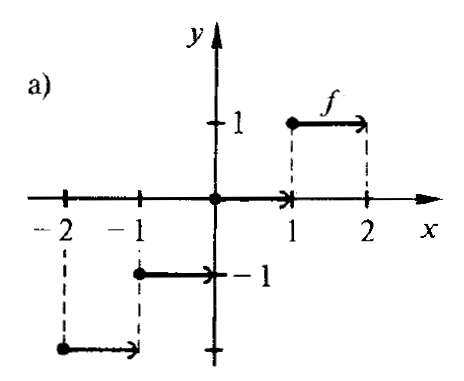
\includegraphics[height=3cm]{Bilder/floor-funktion} & &   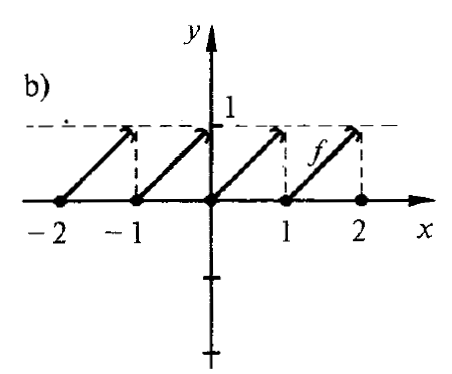
\includegraphics[height=3cm]{Bilder/saegezahn-funktion} \\
			Schreibweise: \textbf{$[x]$} & &  Schreibweise: \textbf{$x - [x]$}
			\end{tabular}

            \columnbreak
			
			\subsubsection{Schwingungen}
			Sinus-Schwingung:  $y = A \cdot \sin(\omega \, t + \phi)$ \\
			\\
			\begin{tabular}{llllllll}
			$A$ & Amplitude & & 
			$\omega$ & Frequenz $\frac{2 \pi}{\mathrm{sec}}$ & & $\varphi$ & Phase \\
			\end{tabular}						
			\\
			
			
			\paragraph{Superposition von Schwingungen} 
			$y = A \cdot \sin(\omega \, t + \varphi)  =  A_1 + A_2 \cdot \sin(\omega \, t + \varphi_1 + \varphi_2)$\\ 
			\\
			$A = \sqrt{A_1^2 + A_2^2 + 2 \,A_1 \cdot A_2 \cdot \cos(\varphi_1 - \varphi_2)}$
			
			
			\subsubsection{Verkettung oder mittelbare Funktion}
			\begin{tabular}{ll} % Tabelle mit 2 Sptalten
			g nach f: & \\
			$h(x)=g \circ f \Rightarrow h(x)=g(f(x))$ & $W_h=W_g \rightarrow D_h=D_f$ \\
			\\
			f nach g: \\
			$h(x)=f \circ g \Rightarrow h(x)=f(g(x))$ & $W_h=W_f \rightarrow D_h=D_g$				
			\end{tabular}
			
			
			\subsubsection{Gerade / ungerade Funktionen}
				\begin{tabular}{lll} 
				 gerade: & $f(-x) = f(x)$ & symmetrisch zu y-Achse \\
				 ungerade: & $f(-x) = -f(x)$ & punktsymmetrisch \\
				 periodisch: & $f(x) = f(x \pm p)$ & wiederholend mit Periode p \\								
				\end{tabular}			
			
			
			\subsubsection{Ganzrationale Funtkionen (Polynome)}

			Aussehen: $f(x)=a_nx^{n}+a_{n-1}x^{n-1}+\cdots+a_1x+a_0$\\
			\\
			Nullstellen bestimmen:
			\\
			Quadratische Funktion: $x_1 , x_2 = \frac{-b \pm \sqrt{b^2 - 4ac}}{2a}$ \\
			\\
			Faktorisierung mit Binomen / Hornerschema \\
			\\
			Eine Funktion vom Grad n hat höchstens n verschiedene Nullstellen!
			
			
			\subsubsection{Gebrochenrationale Funktionen}
			Aussehen: $f(x)=\frac{p_m(x)}{q_n(x)}=\frac{a_mx^{m}+a_{m-1}x^{m-1}+\cdots+a_1x+a_0}{a_nx^{n}+a_{n-1}x^{n-1}+\cdots+a_1x+a_0}$ \\
			\\
			\begin{tabular}{ll} 
				m & Zählergrad \\
				n & Nennergrad \\
				$m < n$ & echt gebrochen \\
				$m = n$ & gleichgradig \\
				$m > n$ & unecht gebrochen\\ 
			\end{tabular}	
			\\
			\\ Jede unecht gebrochene Funktion lässt sich als Summe einer ganzrationalen Funktion und einer echt gebrochenen Funktion schreiben. \\
			$\Rightarrow$ Polynomdivision \\
			
            \columnbreak
			
			\subsubsection{Hornerschema}
			Zerlegt eine ganzrationale Funktion vom Grad n in einen Linearfaktor (Nullstelle) und ein Polynom vom Grad n-1 \\
			\\
			\begin{tabular}{ll}
			1. & Nullstelle $x_0$ raten \\
			2. & Von oben nach unten summieren \\
			3. & Diagonal nach rechts mit $x_0$ multiplizieren
			\end{tabular}	
			
			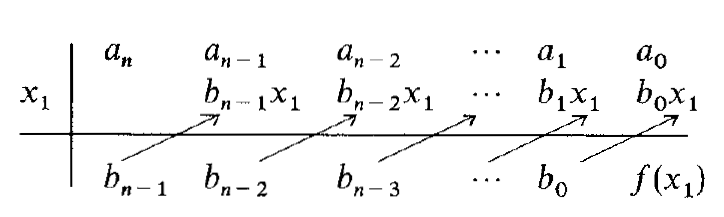
\includegraphics[width=0.7\linewidth]{Bilder/hornerschema_allg}
					

			\textbf{Beispiel:}\\
			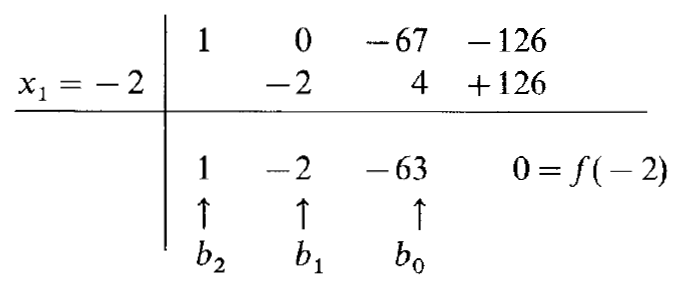
\includegraphics[height=2cm]{Bilder/hornerschema_bsp} \\
			\\
			$f(x) = x^3-67x-126$\\
			% Bild konkretes Hornerschema \\
			$\Rightarrow f(x) = (x-x_1)(b_2x^2 + b_1x + b_0) = (x+2)(x^2-2x-63)$ 
			
			
			\subsubsection{Polynomdivision}
			Liefert Summe aus ganzrationaler Funktion und echt gebrochener Funktion\\
			\\
			\textbf{Beispiel:}\\
			\vspace{-5pt} \polylongdiv[style=C]{-2x^2-x-1}{x-1} \\
			
			
			\subsubsection{Partialbruchzerlegung}
			\begin{tabular}{lll}
			(1) & echt gebrochen ($m < n$) & \\
			 &  Ja: $\rightarrow$ (2) & Nein: $\rightarrow$ Polynomdivision \\
			(2) & Nenner faktorisieren & \\
			 & pro Faktor ein Teilbruch & \\
			(3) & Berechnung Zählerkonstanten & \\
			(3.1) & Gleichnahmig machen (kgV) & \\
			(3.2) & Zählergleichung &\\
			(3.3) & Einsetzen von "guten"  x-Werten &\\			
			\end{tabular}
			
			\paragraph{Beispiel PBZ}
			
			\begin{tabular}{ll}
			(1) & $f(x) = \frac{1}{a^2 - x^2}$ \\
			\\
			(2) & $a^2 - x^2 = (a+x)(a-x)$ \\
			\\
			(3) & $\frac{A}{a+x} + \frac{B}{a-x} = \frac{1}{a^2 - x^2}$\\
			\\
			(3.1) & $\frac{A(a-x) + B(a+x)}{a^2 - x^2} = \frac{1}{a^2 - x^2}$ \\
			\\
			(3.2) &$ A(a-x) + B(a+x) = 1$ \\
			\\
			(3.3) & $x = a \Rightarrow B(2a) = 1 \Rightarrow B = \frac{1}{2a} $ \\			
			& $x = -a \Rightarrow A(2a) = 1 \Rightarrow A = \frac{1}{2a} $ \\
			\end{tabular}
		
		
			\paragraph{Spezielle Ansätze PBZ}
			\begin{tabular}{ll}
			$f(x)$ & $=\frac{5x^2-37x+54}{x^3-6x^2+9x} =  \frac{A}{x}+\frac{B}{x-3}+\frac{C}{(x-3)^2}$ \\ 					 			& $=\frac{A(x-3)^2+Bx(x-3)+Cx}{x(x-3)^2}$ \\
			\\
			$f(x)$ & $=\frac{1,5x}{x^3-6x^2+12x-8}=\frac{A}{x-2}+\frac{B}{(x-2)^2}+\frac{C}{(x-2)^3}$ \\		 			    & $=\frac{A(x-2)^2+B(x-2)+C}{(x-2)^3}$ \\
			\\
			$f(x)$ & $=\frac{x^2-1}{x^3+2x^2-2x-12}=\frac{A}{x-2}+\frac{Bx+C}{x^2+4x+6}$ \\
			& $=\frac{A(x^2+4x+6)+(Bx+C)(x-2)}{(x-2)(x^2+4x+6)}$ \\
			\end{tabular}
		
			
			\subsubsection{Trigonometrie, Arcus}
			\begin{tabular}{llll}
			$\sin(x)$: & $D_f=[-\frac{\pi}{2},\frac{\pi}{2}]$ & $\rightarrow$ &  $W_f=[-1,1]$ \\
			$\cos(x)$: & $D_f=[0,\pi]$ & $\rightarrow$ &  $W_f=[-1,1]$  \\
			$\tan(x)$: & $D_f=(-\frac{\pi}{2},\frac{\pi}{2})$ & $\rightarrow$ & $W_f=\mathbb{R}$\\
			$\cot(x)$: & $D_f=(0,\pi)$ & $\rightarrow$ &  $W_f=\mathbb{R}$ \\
			\\
			$\arcsin(x)$: & $D_f=[-1,1] $ & $\rightarrow$ & $ W_f=[-\frac{\pi}{2},\frac{\pi}{2}]$ \\
			$\arccos(x)$: & $D_f=[-1,1]$ & $\rightarrow$ &  $W_f=[0,\pi]$ \\
			$\arctan(x)$: & $D_f=\mathbb{R}$ & $\rightarrow$ &  $W_f=(-\frac{\pi}{2},\frac{\pi}{2})$ \\
			$\mathrm{arccot}(x)$: & $D_f=[-1,1]$ & $\rightarrow$ &  $W_f=(0,\pi)$ \\		
			\end{tabular}


			\paragraph{Umwandlung}
			\begin{tabular}{ll}
			$\sin(x + \frac{\pi}{2}) = \cos(x)$ & $\cos(x - \frac{\pi}{2}) = \sin(x)$ \\	
			\end{tabular}
			
			
			\paragraph{Symmetrien} 
			\begin{tabular}{ll}
			 Sinus & \\
			  & Punkt $(0|0) \rightarrow \sin(-x) = - \sin(x)$ \\
			  & Scheitelsymm. $\rightarrow \sin(\frac{\pi}{2} + x) = \sin(\frac{\pi}{2} - x)$ \\
			  & Punkt $\rightarrow \sin(\pi - x) = \sin(x)$ \\
			  Cosinus & \\
			  & y-Achse $\rightarrow \cos(-x) = \cos(x)$ \\
			  & Scheitel $\rightarrow \cos(\pi - x) = \cos(\pi + x)$ \\		
			\end{tabular}
			
			
			\subsubsection{Winkel zwischen beliebigen Geraden}
			\begin{tabular}{ll}
			Zwischenwinkel: & $\tan(\alpha) = \frac{m_1 - m_2}{1 + m_1 \cdot m_2} \rightarrow$ Winkel geg. Uhrzeiger \\
			& 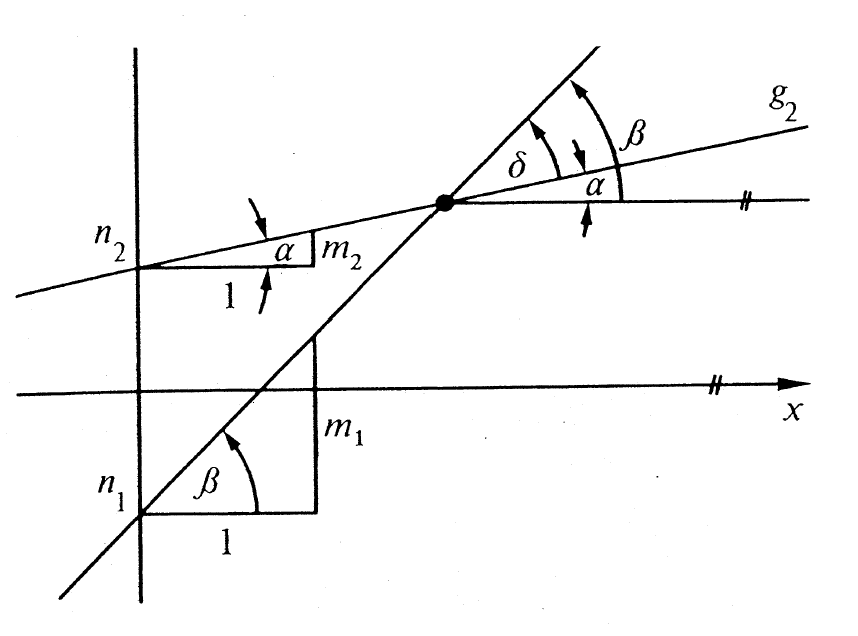
\includegraphics[width=0.3\linewidth]{Bilder/zwischenwinkel.png}\\
			Senkr. Geraden: & $m_1 \cdot m_2 = -1$ \\
			\end{tabular}
            
		
		
		
		\subsection{Folgen und Reihen}			
			
			\subsubsection{Spezielle Folgen und Reihen}
			\begin{tabular}{lll}
			Arithmetische Folge: & $a_{n+1} = a_n + d$ & $d = a_{n+1} - a_n$ \\
			\\
			Geometrische Folge: & $a_{n+1} = q \cdot a_n $ & $q = \frac{a_{n+1}}{a_n}$ \\
			\\
			Konstante Folge: & $a_{n+1} = a_n$  & \\
			\end{tabular}				
			
			
			\subsubsection{Beschränktheit / Monotonie}
			\paragraph{Beschränktheit}
			$W_f \subset [a ; b]$ und a, b $\in \mathbb{R}$		
			
			
			\paragraph{Monotonie}
			
			\begin{tabular}{|c|c|c|c|}
				\hline
				$f(x_1) \leq f(x_2)$ & $x_1 < x_2$ & monoton wachsend & $\uparrow$\\
				\hline
				$f(x_1) < f(x_2)$ & $x_1 < x_2$ & streng monoton wachsend & $\Uparrow$\\
				\hline
				$f(x_1) \geq f(x_2)$ & $x_1 > x_2$ & monoton fallend & $\downarrow$\\
				\hline
				$f(x_1) > f(x_2)$ & $x_1 > x_2$ & streng monoton fallend & $\Downarrow$\\
				\hline
			\end{tabular}
			
			
			\subsubsection{Konvergenz, Divergenz}
				\paragraph{Konvergenz}
			Es existiert ein Grenzwert g $\in \mathbb{R}$	\\
			\\
			Toleranzungleichung: $\vert a_n - g \vert < \epsilon$  mit $\epsilon > 0$ \\
			\\
			Gesucht ist ein $n_0$, ab welchem alle Werte von $n \geq n_0$ in $U_\epsilon(g)$ liegen 
			
			\paragraph{Bestimmt divergent gegen +$\infty$}				Ungleichung: $f_n > K$ wenn $n \geq  n_0$ f"ur $K > 0$ 
			
			\paragraph{Bestimmt divergent gegen -$\infty$}
			Ungleichung: $f_n < k$ wenn $n \geq  n_0$ f"ur $k < 0$ 
			
			\paragraph{Unbestimmt divergent}
			Alles, was nicht konvergent oder bestimmt divergent ist
			
			
			\subsubsection{Grenzwerte gegen Unendlich}
			Vorgehen beim lösen von Grenzwerten \\
			\begin{tabular}{ll}
			1. & Naiven Ansatz ausprobieren $\rightarrow$ limit direkt bilden \\
			2. & Falls unbestimmte Form entsteht: \\
			& Umformen gemäss folgenden Ans"atzen \\
			\end{tabular}
			\\
			
			\begin{tabular}{ll}
			Arithmetik: & $+, -, *, :, \sqrt{...}, \vert ...\vert$ \\
			Erweiterung:& erweitern mit $\frac{1}{x^n}$ n = h"ochste (Nenner-)Potenz \\
			Erweiterung: & erweitern mit Gegentherm (3. Binom bilden)\\
			Tabelle: & Bei Br"uchen Tabelle aus Abschnitt 4.8 anschauen! \\
			\end{tabular}

				\paragraph{Beispiel Grenzwert n gegen Unendlich}
				$f(n) = \frac{-2n^2+4n-5}{8n^2-3n+7}$ $(n \rightarrow \infty)$ \\
				\\
				"Naiv": $\frac{-\infty + \infty + 5}{\infty - \infty + 7} \rightarrow \frac{-\infty + \infty}{\infty - \infty} \rightarrow \frac{?}{?}$ \\
				\\
				Algebra, Erweitern mit $\frac{1}{n^2}$: $f(n) = \frac{-2+\frac{4}{n}-\frac{5}{n^2}}{8-\frac{3}{n}+\frac{7}{n^2}} (n \rightarrow \infty) = \frac{-2}{8} = -\frac{1}{4}$ \\
				
		
			\subsubsection{Rechnen mit Unendlich}
				\paragraph{Bestimmte Formen}
				\begin{tabular}{lll}
				$\infty + \infty = \infty$ & $-\infty - \infty = -\infty$ & $0 \cdot [a,b] = 0 \cdot \text{beschr"ankt} = 0$ \\
				\\
				$g + \infty = \infty$ & $g - \infty = -\infty$ & 	(g $\in \mathbb{R})$ \\
				\\ 
				$\infty \cdot \infty = \infty$ &	$-\infty \cdot (\infty) = -\infty$ & $g \cdot \infty = \begin{cases}
											\infty & g > 0 \\ 
											-\infty & g < 0 
											\end{cases}$\\ 		
				\\
				$\frac{1}{\infty} = 0$ &	$\frac{g}{\infty} = 0$ & 	$g \in \mathbb{R}$	\\
				\\
				$\frac{\infty}{0+} = \infty$	& $\frac{\infty}{0-} = -\infty$	& $\frac{\infty}{g}$ = 	$\begin{cases}			
										\infty & g > 0 \\
										-\infty & g < 0
										\end{cases} $ \\
				\\
				$\frac{1}{0+} = \infty$ & $\frac{1}{0-} = -\infty$	 & $g \in \mathbb{R} - {0}$\\
				\end{tabular}
				\\
				\begin{tabular}{ll}
				$\frac{g}{0+} = 	\begin{cases}					
								\infty & g > 0 \\
								-\infty & g < 0
								\end{cases} $ &
				$\frac{g}{0-} = 	\begin{cases}				
								-\infty & g > 0 \\
								\infty & g < 0
								\end{cases}$ \\ 
				\end{tabular}
				

				\paragraph{Unbestimmte Formen}
				\begin{tabular}{lll}
				$\frac{0}{0} = ?$ & $\frac{\infty}{\infty} = ?$ & $\infty \cdot 0 = ?$ \\
				\\
				$0 \cdot \infty = ?$ & $\infty - \infty = ?$ & $0^0 = ?$ \\
				\\
				$\infty^0 = ?$ & $1^{\infty} = ?$ & \\
	
				\end{tabular}
			
			Ausser 1 ist eine Konstante, dann gilt $1^{\infty} = 1 $ \\
			
			
			\subsubsection{Einschliessung}  % Zum Platz sparen zusammenlegen mit Grenzwerten gegen Unendlich
			Es existieren drei Folgen : $O_n, f_n$ und $U_n$\\
			Es gilt: $O_n \geq f_n \geq U_n$ \\
			
			WENN $O_n$ gegen Grenzwert g konverviert UND $U_n$ ebenfalls gegen g konvergiert, DANN konvergiert auch  $f_n$ gegen g \\ 
		
			
			\subsubsection{Wachstumsvergleich} 
			\begin{tabular}{lll}
			(1) & $\frac{n^k}{q^n} (n \rightarrow \infty)= 0$  (k $\in \mathbb{N}; q > 1)$ & $\frac{\text{Potenz}}{\text{Exponentiell}} \rightarrow 0$\\
			\\
			(2) & $\frac{q^n}{n!} (n \rightarrow \infty)= 0$  (k $\in \mathbb{N}; q > 1)$ & $\frac{\text{Exponentiell}}{\text{Fakult"at}} \rightarrow 0$ \\
			\\
			(2) & $\frac{ln(n)}{n^k} (n \rightarrow \infty)= 0$  (k $\in \mathbb{N})$ & $\frac{\text{Logarithmisch}}{\text{Potenz}} \rightarrow 0$ \\
			\\
			\end{tabular}						
			
			
			\subsubsection{Bolzano-Prinzip}
			\textbf{Jede beschränkte, monotone Zahlenfolge ist konvergent!} \\
			\begin{tabular}{ll}
			1. & Monotonie beweisen \\
			2. &  Beschränktheit vermuten und möglichen Grenzwert g \\ 
			& mittels Grenzwertgleichung finden  \\
			3. & Beschränktheit beweisen \\
			3.1 & $a_1$ ist obere/untere Schranke \\
			3.2 & Vermutete untere/obere Schranke mit voll. Induktion beweisen \\
			& z.B. $a_{n+1} \leq a_n$ wobei $a_{n+1}$ und $a_n$ mit vermutetem \\
			& Grenzwert ersetzt werden
			\end{tabular}
			

			
			\subsubsection{Exponentialfunktion}
			$\e = \lim\limits_{n \to \infty} (1+\frac{1}{n})^n $ \\
			\\
			\begin{minipage}{.45\linewidth}
			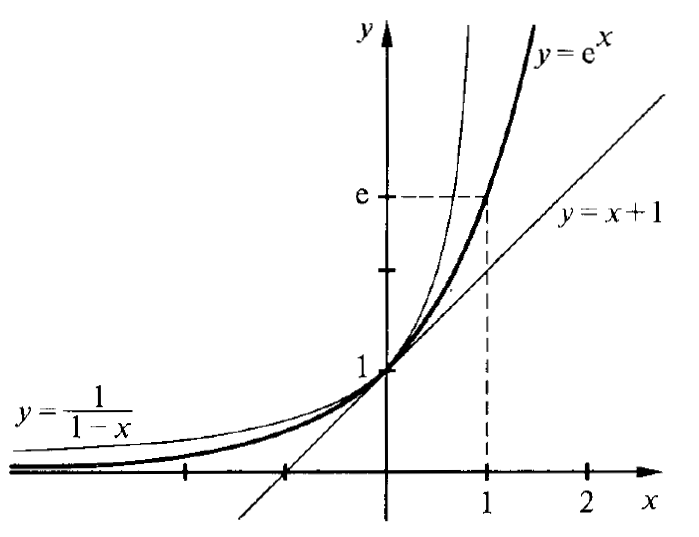
\includegraphics[width=0.95\linewidth]{Bilder/exp-funktion}
			
			\end{minipage}
			\hfill
			\begin{minipage}{.5\linewidth}
			Definitions- / Wertebereich: \\
			\\
			$D_f = \mathbb{R} \rightarrow W_f = \mathbb{R^+}$ \\
			\\
			Einschliessung: \\
			\\
			\begin{tabular}{ll}
			$\e^x \geq 1 + x$ & f"ur x $\in \mathbb{R}$ \\
			\\
			$\e^x \leq \frac{1}{1-x}$ & f"ur $x < 1$  \\
			\end{tabular}
			\end{minipage}
			
			
			
			\subsubsection{Hyperbolische Funktionen}
			$\e^x = \frac{1}{2} (\e^x - \e^{-x}) + \frac{1}{2} (\e^x + \e^{-x}) = \sinh(x) + \cosh(x)$ \\
			\\
			\begin{tabular}{ll}
			$\sinh(x) = \frac{1}{2} (\e^x - \e^{-x})$ & $\mathbb{R} \rightarrow \mathbb{R}$ \\
			$\cosh(x) = \frac{1}{2} (\e^x + \e^{-x})$ & $\mathbb{R} \rightarrow [1; \infty)$ \\
			$\tanh(x)$ = $\frac{\sinh(x)}{\cosh(x)} = \frac{\frac{1}{2} (\e^x - \e^{-x})}{\frac{1}{2} (\e^x + \e^{-x})}$ & $\mathbb{R} \rightarrow (-1; 1)$ \\	
		
			$\vert \sinh(x) \vert < \cosh(x)$	& \\
			\end{tabular}
			
			
			\paragraph{Area-Funktionen (Umkehrung Hyperbolische. F.)}
			\begin{tabular}{ll}
			$\mathrm{arsinh}(x): $ &  $\mathbb{R} \rightarrow \mathbb{R}$ \\
			$\mathrm{arcosh}(x): $ & $[1; \infty) \rightarrow \mathbb{R}^+_0$  \\
			$\mathrm{artanh}(x): $ & $ \vert x \vert < 1 \rightarrow \mathbb{R} $ \\
			
			\end{tabular}
			
			
			\subsubsection{Logarithmusfunktion}
				
			\begin{minipage}{.45\linewidth}
			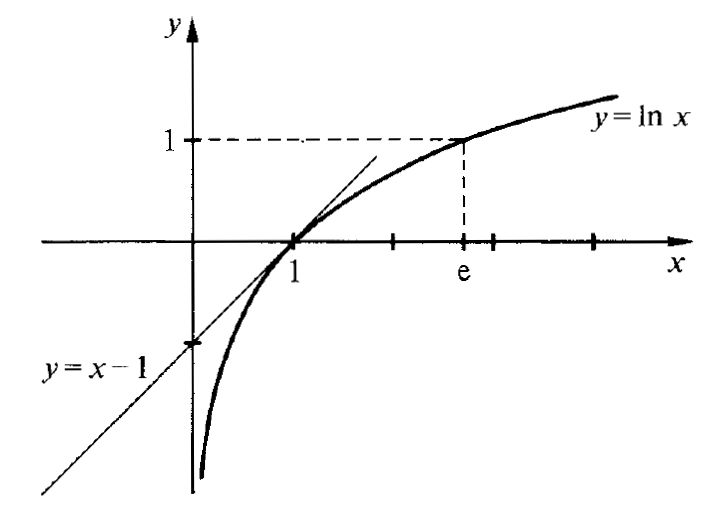
\includegraphics[width=0.95\linewidth]{Bilder/ln-funktion}
			\end{minipage}
			\hfill
			\begin{minipage}{.5\linewidth}
			Definitions- / Wertebereich: \\
			$D_f = \mathbb{R^+} \rightarrow W_f = \mathbb{R}$ \\
			\\
			Einschliessung: \\
			\\
			$1-\frac{1}{x} \leq \ln(x) \leq x-1$
			\end{minipage}
				
			
			
			
		\subsection{Grenzwerte von Funktionen}
			\begin{tabular}{llll}
			Grenzwertsätze & S. 56-57 & & \\
			\end{tabular}
			
			\subsubsection{Techniken zur Berechnung von Grenzwerten}	
			\begin{tabular}{ll}
			Arithmetik: & $+, -, *, :, \sqrt{...}, \vert ...\vert$ \\
			Erweiterung:& erweitern mit $\frac{1}{x^n}$ n = h"ochste (Nenner-)Potenz \\
			Erweiterung: & erweitern mit Gegentherm (3. Binom bilden)\\
			Faktorisierung: & Z"ahler und Nenner faktoriesieren und kürzen \\
			\textbf{Trigo:} & \textbf{Bronstein S. 57 1. C beachten}
			\end{tabular}
			
			
			\subsubsection{Links- / Rechtsseitiger Grenzwert}
			Eine kritische Stelle $x_0$ 	kann von links und rechts angen"ahert werden. \\
			
			\begin{tabular}{ll}
			linksseitiger Grenzwert: & $\lim\limits_{x \to x_0^-} f(x) = g^-$ \\
			\\
			rechtsseitiger Grenzwert: & $\lim\limits_{x \to x_0^+} f(x) = g^+$ \\
			\end{tabular}
			\\ 
			$\Rightarrow$ Wenn $g^- = g^+ = g \rightarrow$ Konvergenz  \\
			$\Rightarrow$ Wenn $g^- \neq g^+ \rightarrow$ unbestimmte Divergenz \\


			\subsubsection{Konvergenz, Divergenz}	
				\paragraph{Konvergenz von f(x)}
			
			\begin{tabular}{lll}
			$x \rightarrow \infty$ & Toleranzungleichung: $\vert f(x) - g \vert < \epsilon$ & wenn $x > M(\epsilon)$ \\
			$x \rightarrow -\infty$ & Toleranzungleichung: $\vert f(x) - g \vert < \epsilon$ & wenn $x < m(\epsilon)$ \\
			\\
			$x \rightarrow x_0$ & Toleranzungleichung:  $\vert f(x) - g \vert < \epsilon$ & $ x \in \dot{U}_\delta(x_0)$ \\
			\end{tabular}

			
			\paragraph{Bestimmte Divergenz von y = f(x)}
			\begin{tabular}{lll}
			Quadrant & Kriterium & Folgerung  \\
			\Romannum{1}	 & 	$y \rightarrow \infty$ $(x \rightarrow \infty$) & $y > K$ wenn $x > M(K)$ \\
			 \Romannum{2}	 & 	$y \rightarrow \infty$ $(x \rightarrow -\infty$) & $y > K$ wenn $x < m(K)$ \\
			 \Romannum{3}	 & 	$y \rightarrow -\infty$ $(x \rightarrow -\infty$) & $y < k$ wenn $x < m(k)$ \\
			 \Romannum{4}	 & 	$y \rightarrow -\infty$ $(x \rightarrow \infty$) & $y < k$ wenn $x > M(k)$ \\
			\\
			& 	$f(x) \rightarrow \infty$ & $y > K > 0$ wenn $ x \in \dot{U}_\delta(x_0)$ \\
			& 	$f(x) \rightarrow -\infty$ & $y < k < 0$ wenn $ x \in \dot{U}_\delta(x_0)$ \\
			\end{tabular}
		
			
			\subsubsection{Stetigkeit}
			Definition Stetigkeit: $\lim \limits_{x \to x_0} f(x) = f(x_0)$ \\
			Eine Funktion ist stetig, wenn der Funktionsgraph kann gezeichnet werden, ohne dass der Stift abgesetzt werden muss. \\
			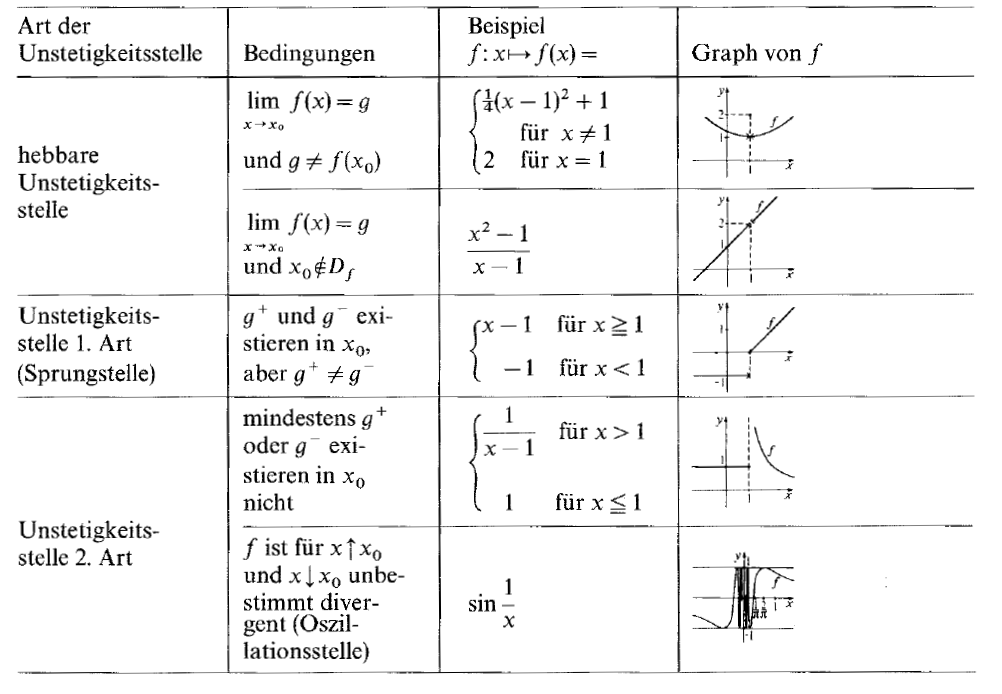
\includegraphics[width=0.9\linewidth]{Bilder/stetigkeit} \\


			\subsubsection{"Ubertragungsprinzip (Folgenprinzip)}
			f bestitz an der Stelle $x_0$ Grenzwert g, wenn für jede gegen $x_0$\\
		    konvergente Folge $< x_n >$ gilt: $\lim\limits_{x \to \infty} f(x_n) = g$ 
		    
			\paragraph{Beispiel}
			$f(x) = \frac{\vert x + 2 \vert}{2x+4}$ und $x_0 = -2$ \\
			\begin{tabular}{ll}
			linksseitig: & $x_n = x_0 - \frac{1}{n}$ für jedes x in f(x) einsetzen; \\
			 & Grenzwert $g^-$ gegen $\infty$ bestimmen \\
			\\
			rechtsseitig: & $x_n = x_0 + \frac{1}{n}$ für jedes x in f(x) einsetzen; \\
			& Grenzwert $g^+$ gegen $\infty$ bestimmen \\
			\end{tabular}
			
			
			\subsubsection{Nullstellen bestimmen gem"ass Bolzano}
			$f(x)$ auf Intervall $[a;b]$ stetig und $f(a)$ und $f(b)$ versch. Vorzeichen \\
			$\rightarrow$ Es existiert (mindestens) eine 	Nullstelle $\xi$\\	
			NS mittels Bisektion (Intervallschachtelung) näherungsweise berechnen: \\
			
			\begin{tabular}{ll}
			(1) & $I_0 = [a ; b] = [a_0 ; b_0]$ gesamtes Intervall \\
			(2) & $I_0$ halbieren $\rightarrow m = \frac{a_0 + b_0}{2}$ \\
			(3) & Teil-Intervall mit Vorzeichenwechsel bestimmen: \\
			& links: $f(a) \cdot f(m) < 0$ ; rechts: $f(a) \cdot f(m) > 0$ \\
			(4)& Teil-Intervall mit Vorzeichenwechsel: $I_1 = [a_1 ; b_1]$ \\
			(5) & Schritt (2) - (4) n mal wiederholen: $I_{n+1} \in I_n$ \\
			(6) & ... $\xi \in (a;b)$ mit $f(\xi) = 0$ (Nullstelle) \\
			\end{tabular}						
			
		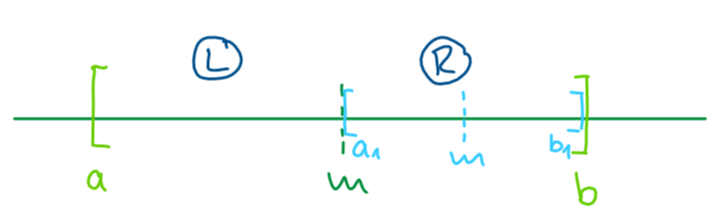
\includegraphics[width=0.9\linewidth]{Bilder/bisektion}
						
			
			\subsubsection{Spezielle Grenzwerte}	
			\begin{tabular}{lll}
			$\lim\limits_{x \to \infty} \frac{\sin(x)}{x} = 1$ &  $\lim\limits_{x \to \infty} (1 + \frac{a}{x})^x = \e^a$ & $\lim\limits_{x \to 0} \frac{\log_a(x+1)}{x} = \frac{1}{\ln(a)}$  \\
			\\
				$\lim\limits_{x \to 1} \frac{x}{1-\e^{-x}} = 1$ & $\lim\limits_{x \to \infty} \sqrt[x]{x} = 1$  & $\lim\limits_{x \to 0} (1+x)^{\frac{1}{x}} = 1$ \\
				\\
			$\lim\limits_{x \to \infty} \frac{(\ln(x))^\alpha}{x^\beta} = 0$ & $\lim\limits_{x \to 0^+} x \cdot \ln(x) = 0$  & $\lim\limits_{x \to 0} \frac{a^x -1}{x} = \ln(a)$ \\
			\\
			$\lim\limits_{x \to 0} \frac{\e^x - 1}{x} = 1$ & $\lim\limits_{x \to 0} \frac{(a+x)^\alpha -1}{x} = \alpha$  & $\lim\limits_{x \to 0+} z^z = 1$ \\
			\\
			$\lim\limits_{x \to 0+} x^{\sin(x)} = 1$ & $\lim\limits_{x \to 0+} y^{\beta} (\ln(y))^{\alpha} = 0 $ &  \\
			\end{tabular}
			\\
			
			\begin{tabular}{ll}
			$\lim\limits_{x \to \infty} \frac{x^\alpha}{a^{\beta x}} = 0 \; (a > 1; \alpha, \beta > 0)$  & $\lim\limits_{x \to \infty} \sum\limits _{k=0}^n q^k = \begin{cases}			
									\infty & q \geq 1 \\
									\frac{1}{1-q} & \vert q \vert < 1
								\end{cases} $ \\ 
			\end{tabular}
					
	
		
			\subsubsection{Asymptotenbestimmung}
			Asymptote einer gebrochen rationalen Funktion $f(x) = \frac{a_nx^n + ... + a_1x + a_0}{b_mx^m + ... + b_1x + b_0}$\\
			 bestimmen gem"ass:
			
			\begin{tabular}{|l|l|l|l|}
			\hline
			 & $m > n$ & $m = n$ & $m < n$ \\
			\hline
			 $\lim\limits_{x\to \pm \infty} r(x)$  & 0 & $\frac{a_n}{b_m}$ & $\infty$ oder $-\infty$ \\
			\hline
			 Asymptote & x-Achse & Parallel zur x-Achse $y = g(x) = \frac{a_m}{b_n}$ & ganzrat. Teil der Polynomdivision\\
			\hline
			 Konv./Div. & Konvergenz & Konvergenz & Divergenz \\
			\hline
			\end{tabular}
			
			
			\subsubsection{Grenzwerte von rekursiven Folgen}
			Anwendung des Bolzano-Prinzips!  Beispiel: $a_1 = \frac{1}{4}$ ; $a_{n+1} = a_n^2 + \frac{1}{4}$ \\
			\\
			\begin{tabular}{ll}
			1. & Monotonie \\
			& beweisen mit Ansatz $a_{n+1} \geq a_n$ bzw. $a_{n+1} \leq a_n$ \\
			\\
			2. & Beschränktheit \\
			& erste Schranke = erster Wert der Reihe \\
			& Zweite Schranke: Annahme, es gibt Grenzwert g und er ist \\
			& sup / inf \\
			\\
			 & Grenzwertgleichung: $a_{n+1} = a_n ^2 + \frac{1}{4}$  $(n \rightarrow \infty)$ $\Rightarrow g = g^2 + \frac{1}{4}$ \\
			 & Gleichung nach g auflösen \\
			 & $\Rightarrow$ Wenn es ein sup / inf gibt, dann ist es das berechnete g $\in \mathbb{R}$\\
			 \\
			 3. & Beweisen (oder widerlegen), dass g sup / inf ist \\
			 & Ansatz: $a_n \leq g$ bzw. $a_n \geq g$ mit vollst. Induktion beweisen \\
			\end{tabular}

	\vfill\null
	\pagebreak

			%Sektion aufgeräumt und strukturell eingeschoben
			%Laut Zgraggen nur 4 Seiten erlaubt, evtl. erst nach Prüfung ausschmücken

		\section{Differentialrechnung S. 444 ff}

				\begin{tabular}{llll} 
				Kurvenuntersuchungen & S. 261 & Taylor-reihe & S. 455 \\
				\end{tabular}
				
				
			\subsection{Begriff der Ableitung / Differenzialquotient S. 444}
			Die Ableitung $f'(x)$ der Funktion $f(x)$ im Punkt $x_0$ entspricht der Steigung der Tangente an	$f(x)$ im Punkt $x_0$		 \\
			\\
			\begin{tabular}{ll}
			Differenzenquotient: & $\frac{f(x + h) - f(x)}{h} = \frac{f(x + \Delta x) - f(x)}{\Delta x}$ \\
			\\
			\textbf{Differenzialquotient:} & $f'(x) = \lim\limits_{\Delta x \to 0} \frac{f(x + \Delta x) - f(x)}{\Delta x}$ \quad $(\Delta x = h)$ \\
			\end{tabular}
			

			\subsection{Tangente / Normale / Zwischenwinkel}
			\begin{tabular}{ll}
			Tangente: & $y = f'(x_0) \cdot (x - x_0) + y_0$ \\
			\\
			Normale: & $y = -\frac{1}{f'(x_0)} \cdot (x - x_0) + y_0$ \\	
			\\
			Zwischenwinkel: &  $tan(\alpha) = \frac{m_1 - m_2}{1 + m_1 \cdot m_2} \rightarrow$ Winkel gegen Uhrz.\\
			\\
			&  $tan(\alpha) =  \frac{m_2 - m_1}{1 + m_1 \cdot m_2} \rightarrow$ Winkel im Uhrzeigersinn\\
			
			\end{tabular}
			
			
			\subsection{Einseitige Ableitungen S. 445}
			rechtsseitig: $f'_r(x_0) = \lim\limits_{x \to x_0^+}f'(x)$ \quad
			linksseitig: $f'_l(x_0) = \lim\limits_{x \to x_0^-}f'(x)$ \\
			\\
			\begin{tabular}{ll}
			$f'_r(x_0) = f'_l(x_0)$ & $\rightarrow$ Konvergenz \\
			Alle anderen Fälle & $\rightarrow$ unbestimmte Divergenz $\rightarrow$ keine Ableitung! \\
			\end{tabular}
			
			

		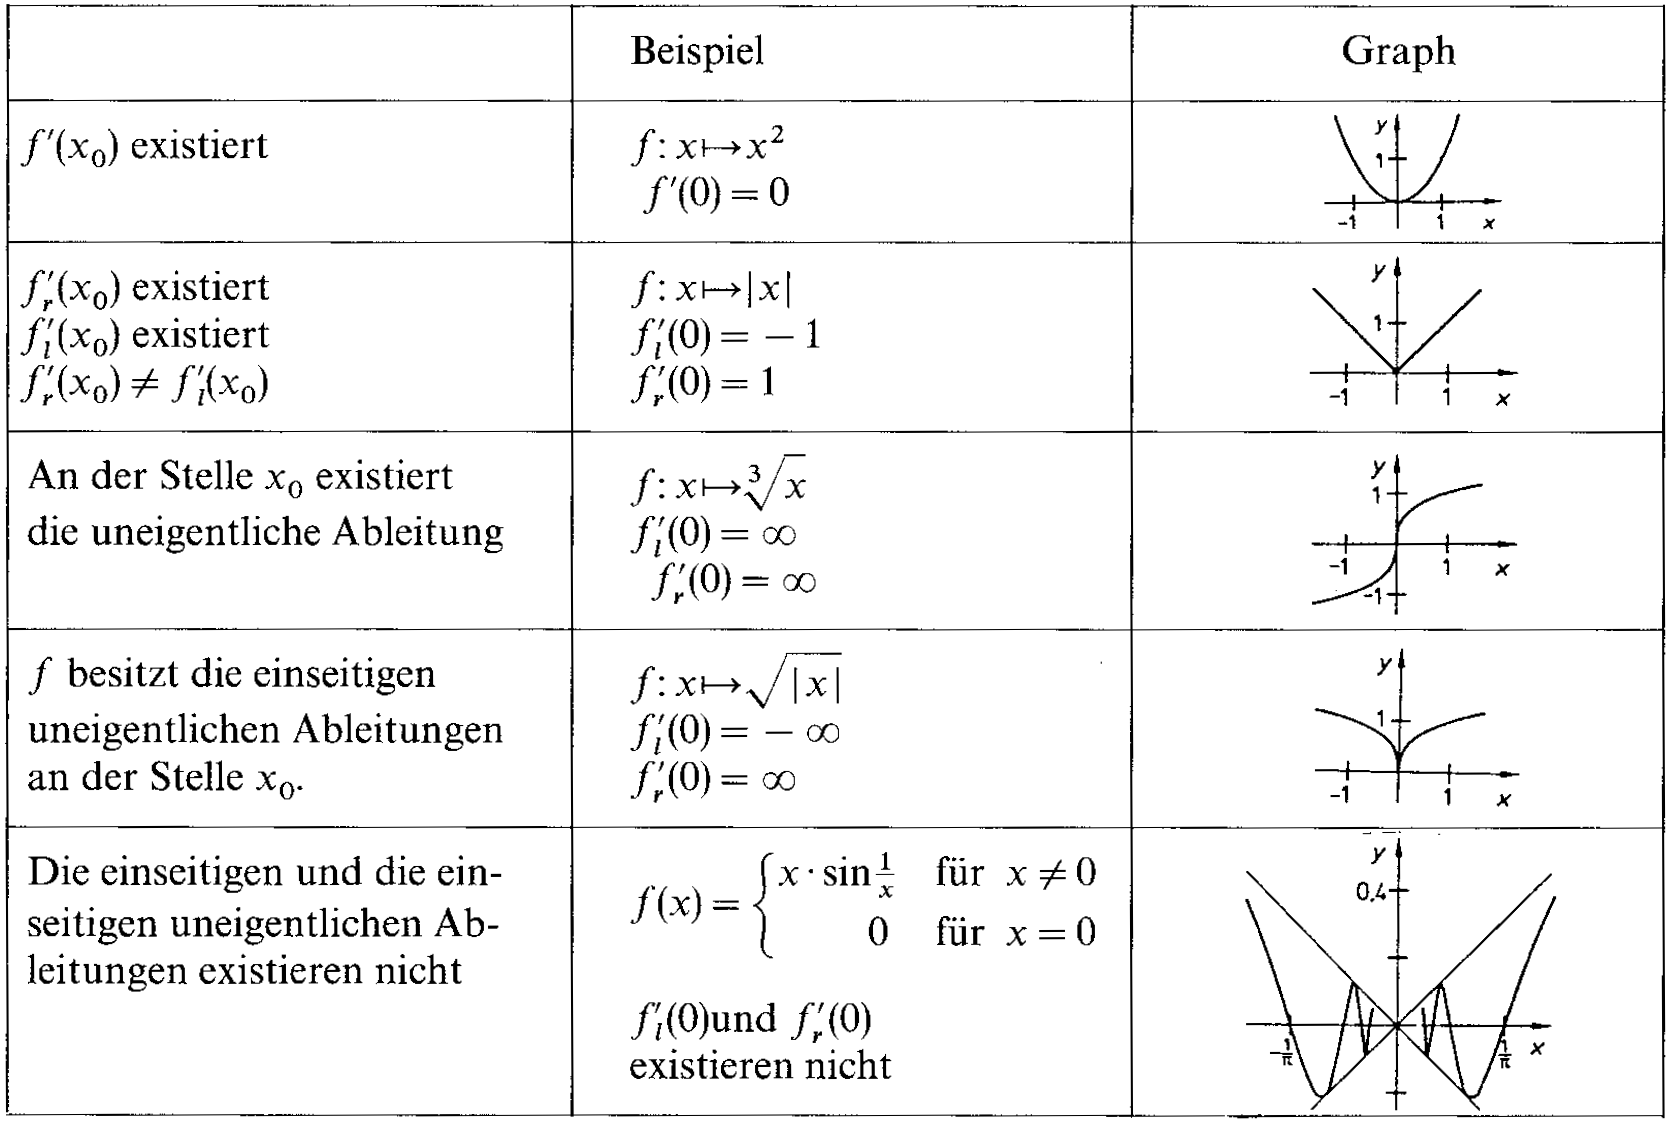
\includegraphics[width=0.9\linewidth]{Bilder/konvergenz-divergenz}
			
			
			\subsection{Generische Muster}
			\begin{tabular}{ll}
			Allg. Potenz &  $\left( f(x)^\alpha \right)' = f'(x) \cdot \alpha \cdot f(x) ^{\alpha - 1} $ \\
			\\
			Allg. log-Regel & $\ln \left( f(x) \right)' = \frac{f'(x)}{f(x)} $ \\
			\\
			Allg. exp-Regel & $ \left( \e^{f(x)} \right)' = f'(x) \cdot \e^{f(x)} $ \\
			\end{tabular}
			
			
			\subsection{Ableitungsregeln S. 445-448}
			
			\subsubsection{Elementare Regeln}
			\begin{tabular}{lll}
			Potenzen: & $f(x) = x^3$ & $f'(x) = 3 \, x^2$ \\
			& $f(x) = x^\alpha$ & $f'(x) = \alpha \cdot x^{\alpha - 1}$ \\
			\\
			Linearität: & $f(x) = c \cdot x^2$ & $f'(x) = c \cdot 2 \, x $ \\
			\\
			Summe: & $(u(x) + v(x) - w(x))' $ & = $u'(x) + v'(x) - w'(x)$ \\
			\\
			Konstanten: & c = konst $\rightarrow$ c' = 0 \\
			\end{tabular}
			
			
			\subsubsection{Produktregel}
			$(f(x) \cdot g(x))' = f'(x) \cdot g(x) + f(x) \cdot g'(x)$ 
			
			\subsubsection{Quotientenregel}
			$\left( \frac{u(x)}{v(x)} \right) ' = \frac{u'(x) \cdot v(x) - u(x) \cdot v'(x)}{v(x) ^2}$ \quad $\rightarrow$ als Produkt schreiben \\
			\\
			$u(x) \cdot \left( \frac{1)}{v(x)} \right) ' =  u'(x) \cdot \frac{1}{v(x)} + u(x) \cdot \frac{- v'(x)}{v(x)^2}$
			
			\subsubsection{Kettenregel}
			$g(f(x))' =  f'(x) \cdot g'(x)$ \\
			
			\subsubsection{Umkehrfunktion}
			$(f^{-1}(y_0))' = \frac{1}{f'(x_0)} =  \frac{1}{f'(f^{-1}(y_0))}$ \\
			

			
			\subsection{Allgemeine Logarithmus-Ableitung}
			$(\log_b(x))' = \left( \frac{\ln(x)}{\ln(b)} \right)' = \frac{1}{\ln(b)} \cdot (\ln(x))' = \frac{1}{\ln(b)} \cdot \frac{1}{x} $
			
			
			\subsection{Lineare Approximation / Differenzial dy S. 459}
			Differenzial = dy = df = "Höhenunterschied der Tangente" \\
			= "Linearzuwachs" \\
			\textcolor{blue}{Differenzial = $f'(x_0) \cdot dx$} $= f'(x_0) \cdot h = f'(x_0) \cdot \Delta x = f'(x_0) \cdot (x- x_0) $ \\
			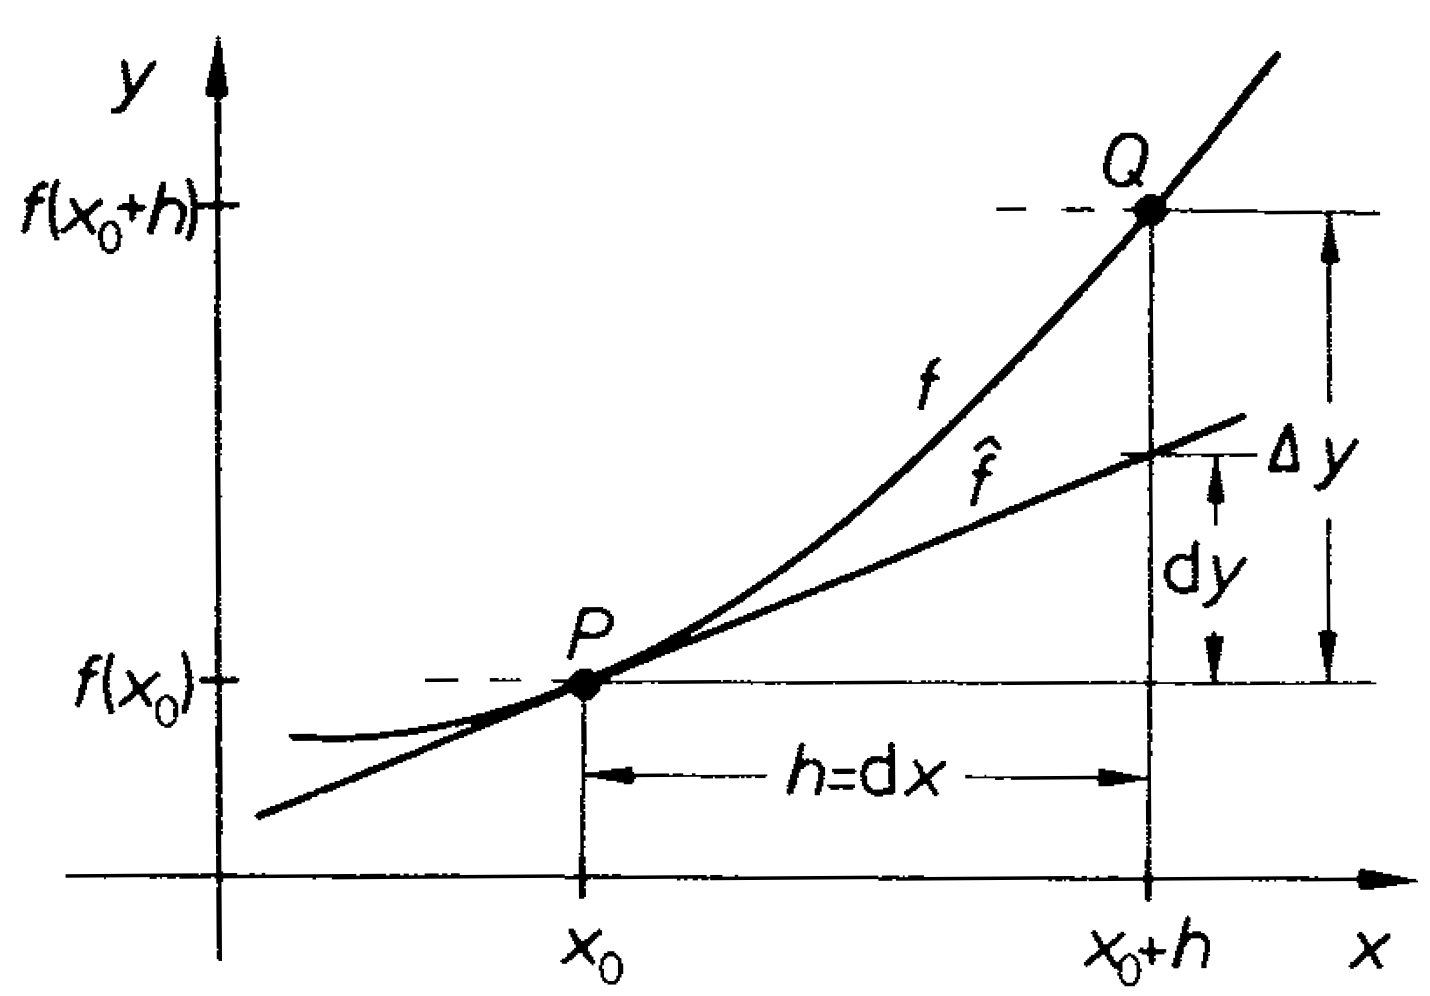
\includegraphics[width=0.8\linewidth]{Bilder/differenzial}  \\
			$\Delta y \approx dy \rightarrow$ Approximation / Fehler \\
			Fehler : \quad $\Delta y - dy \rightarrow 0$ \quad $h \rightarrow 0$ \\	
			\\
			\textbf{Die Tangente ist die beste lineare Approximation!}		
			
			
			\subsection{Approximationsfehler}
			Die Fehler beziehen sich auf den Arbeitspunkt (z.B. $x_0$) \\
			\\
			\begin{tabular}{lll}
			Absoluter Fehler: & $\Delta y - dy = f(x) - \hat f(x)$ & Einheit y \\
			\\
			Relativer Fehler: & $\frac{\Delta y - dy}{y_0} = \frac{f(x) - \hat f(x)}{x_0} $ & Einheitenlos \\
			\end{tabular}
			
			
			\subsection{Fehlerfortpflanzung} 
			\begin{tabular}{llll}
			Absolut: & $\Delta x \rightarrow \Delta y$ & &
			$\Delta y \approx dy = f'(x_0) \cdot dx$ \\
			\\
			Relativ: & $\Delta x \rightarrow \frac{\Delta y}  {y_0}$ & &  $\frac{\Delta y}  {y_0} \approx \frac{dy}{y_0} = \frac{f'(x_0) \cdot dx}{y_0} $ \\
			\end{tabular}
			 \\

			\begin{tabular}{| c | c | c |}
			\hline
			& $\Delta x = dx$ (abs) & $\frac{\Delta x}{x} = \frac{dx}{x}$ (rel)  \\
			\hline
			$\Delta y \approx dy$ (abs) & A & B \\
			\hline
			$\frac{\Delta y}{y} \approx \frac{dy}{y}$ (rel) & C & D \\
			\hline
			\end{tabular}					
			\\ \\
			$\rightarrow$ Tabelle ist bidirektional (Umkehrfunktionen)
			
			
			\subsection{Wichtige Ableitungen S.446}
			
			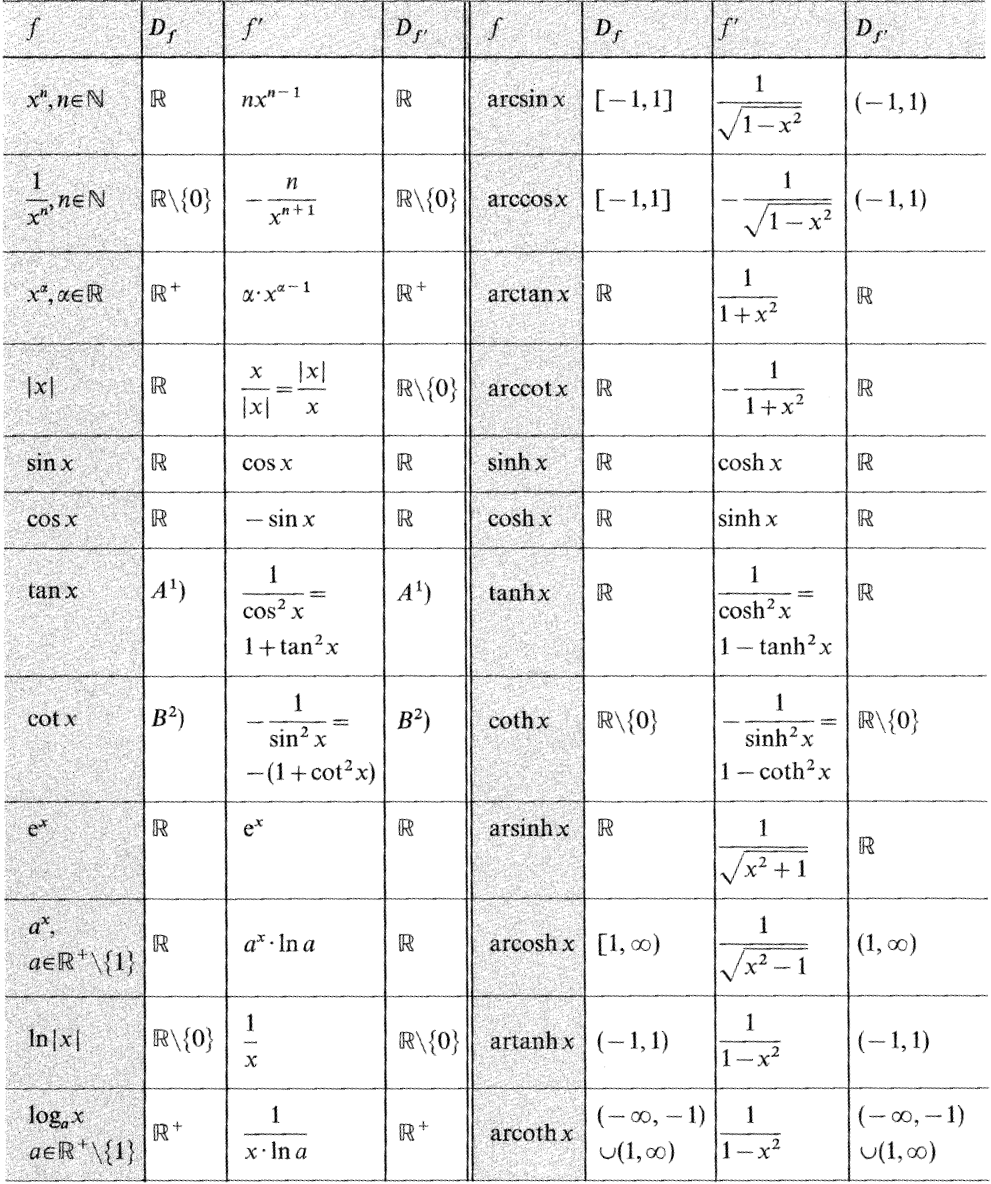
\includegraphics[width=\linewidth]{Bilder/ableitungen}

			
			\subsection{Taylor-Reihe (Approximation höherer Ordnung)}
			n = Ordnung der Approximationsfunktion $p_n(x)$ \\
			$h = x - x_0$ \\
			\\
			$p_n(x) = f(x_0) + f'(x_0) \cdot h + \frac{f''(x_0)}{2!} \cdot h^2 + ... + \frac{f^{(n)}(x_0)}{n!} \cdot h^n$	 \\
			\\
			$p_n(x) = \sum\limits_{k=0}^{n} \frac{f^{(k)}(x_0)}{k!} \cdot h^k \; \vert h = x-x_0$\\
			\\
			Der Approximationsfehler $R_n (x_0, h)$ entspricht $f(x) - p_n(x)$ und wird im nächsten Abschnitt beschrieben.		
			
			
			\subsection{Fehler $R_n$ der Taylor-Reihe}
			Der Fehler ist nicht klar berechenbar, sondern nur auf einem Intervall "bestimmbar" $\rightarrow$ Worst Case! \\			
			Voraussetzung: f auf Intervall [a;b] mind. (n+1) mal ableitbar\\
			\\
			\begin{tabular}{ll}
			\textbf{Lagrange:} &  $\vert R_n \vert = \vert \frac{f^{(n+1)}(\xi)}{(n+1)!} \cdot h^{n+1} \vert $ \\
			\\
			\textbf{Cauchy:} & $\vert R_n \vert = \vert \frac{f^{(n+1)} (\xi)}{n!}  \cdot h^{n+1} \cdot (1 - \theta)^n \vert$ \\
			\\
			& $0 < \theta < 1$    $\xi = x_0 + \theta \cdot h$ \\
			& $\theta$ steuert Lage von $\xi$ auf Intervall \\
			\end{tabular}
			
		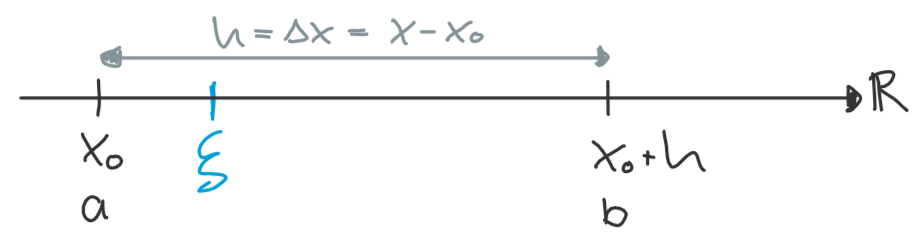
\includegraphics[width=0.7\linewidth]{Bilder/zahlenstrahl}
			
			
			\subsubsection{Verhalten von $R_n$}	
			
			\begin{tabular}{llll}
			1) & $n \rightarrow \infty$ & "Normal" \quad $R_n \rightarrow 0$ & $\vert h \vert$ fix  \\
			2) & $n \rightarrow 0^+$ & "Normal" \quad $R_n \rightarrow 0$ & n fix \\
			& &  $\vert f^{n+1}(\tilde{x})\vert < K^{n+1}$ & $(K < 0, n \in \mathbb{N}_0), \tilde{x} \in (a;b)$ \\
			\end{tabular}
			
			
			\subsection{Satz von Rolle S. 454}
			\begin{tabular}{ll}
			Voraussetzungen: & f auf Intervall [a;b] mind. (n+1) mal ableitbar\\
			 & $f(a) = f(b)$ \\
			\end{tabular}
			
			Auf dem Intervall (a;b) existiert mindestens einmal  eine horizontale Tangente : $f'(\xi) = 0$ \\			
			 \\
			 

			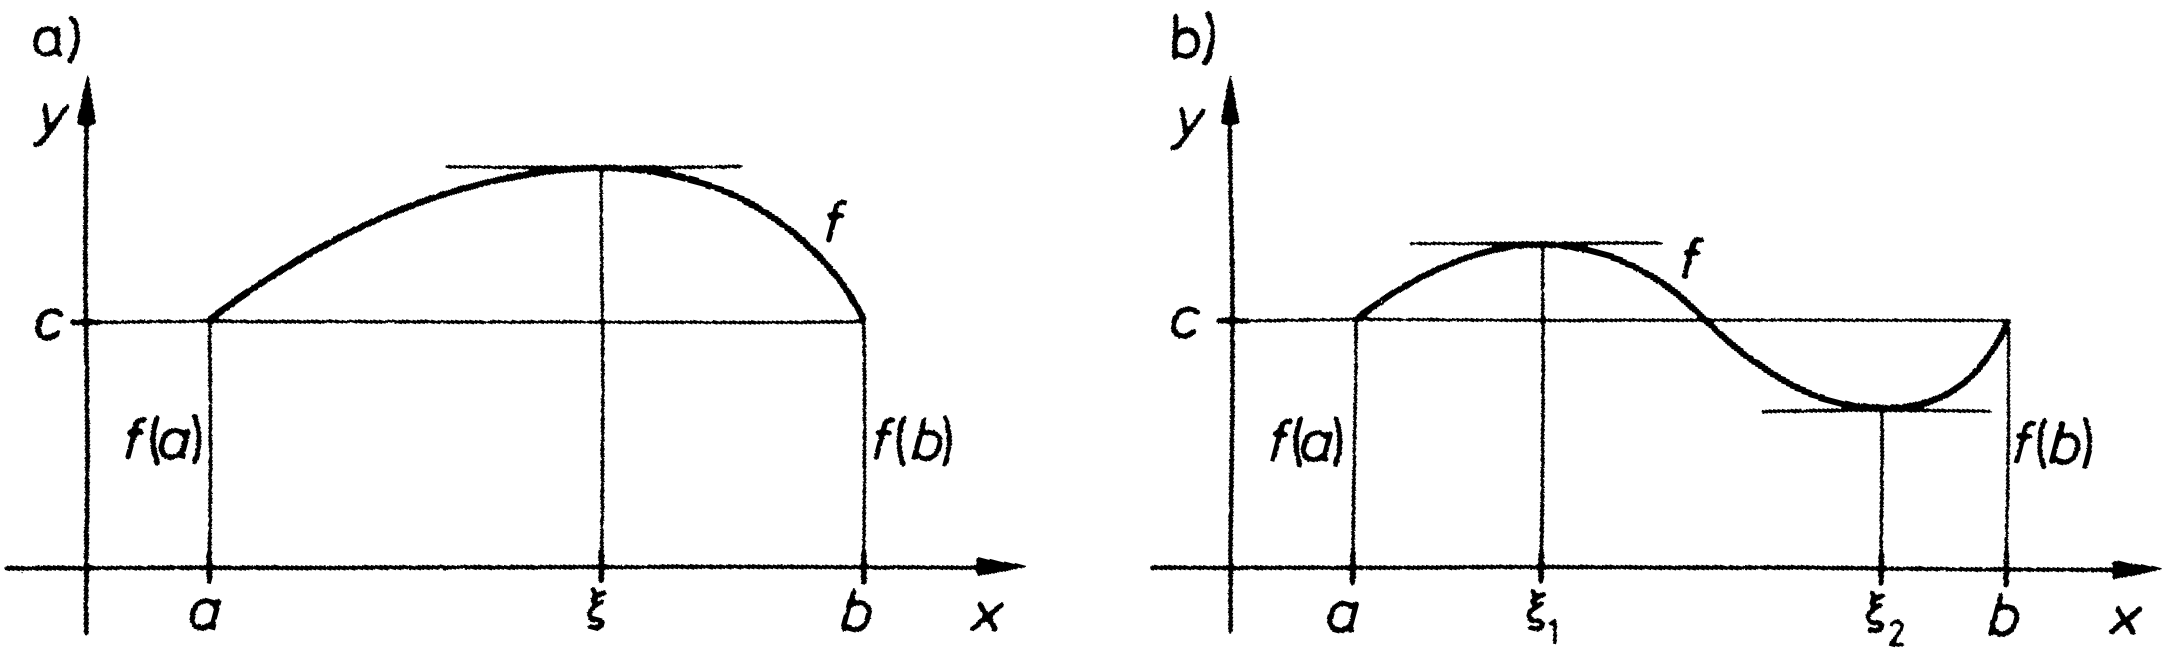
\includegraphics[width=0.9\linewidth]{Bilder/rolle}
			
			
			
			\subsection{Mittelwertsatz S. 454}			
			\begin{tabular}{ll}
			Voraussetzungen: &  f auf Intervall [a;b] mind. (n+1) mal ableitbar \\
			\end{tabular}

			\begin{minipage}[b]{.5\linewidth} 
  			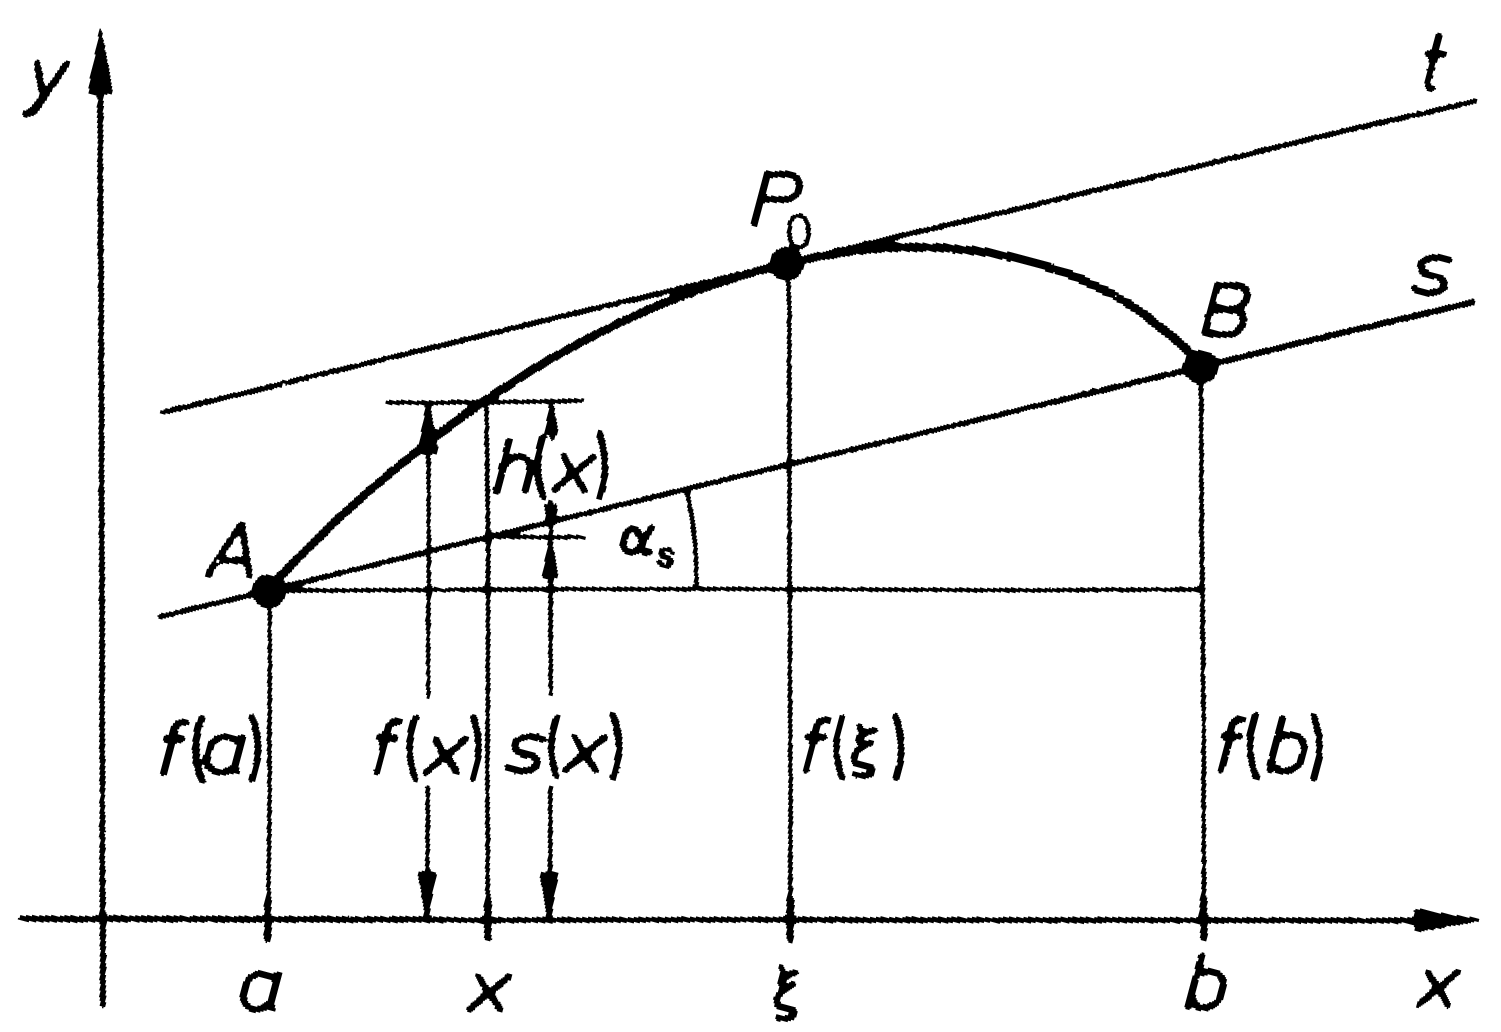
\includegraphics[width=\linewidth]{Bilder/mittelwertsatz}
			\end{minipage}
			\hfill
			\begin{minipage}[b]{.45\linewidth} 
  			
  			Sekantensteigung: \\
  			$m_s = \frac{\Delta y}{\Delta x} = \frac{f(b) - f(a)}{b - a}$ \\
  			\\
  			
  			Tangentensteigung / \\
  			Durchschnittssteigung:
  			$f'(\xi) = \frac{f(b) - f(a)}{b - a}$ \\		
				
			\end{minipage}			
		
			
			\subsection{Extremalstellen S. 455-457}
			f: [a;b] $\rightarrow$ $\mathbb{R}$ , stetig $\Rightarrow W_f$ = abgeschlossenes Intervall 
			
			\subsubsection{Absolut Extremalstelle (Randanalyse durchführen)}
			\begin{tabular}{ll}
			Absolutes Maximum: &  $\mathrm{max}(W_f)$\\
		  	Absolutes Minimum & $\mathrm{min}(W_f)$ \\
			\end{tabular}
			
			\subsubsection{Relative Extremalstelle}
		
			\begin{tabular}{ll}
			Lokales Maximum: & "Berg" (nicht am Rand der Funktion)\\ 
			& $f(x) \leq f(x_0) $ \quad $x \in U_{\delta}(x_0)$  \\
			&Wechsel von $\uparrow$ zu $\downarrow$ \\
			\\
			Lokales Minimum: & "Tal" (nicht am Rand der Funktion)\\
			& $f(x) \geq f(x_0) $ \quad $x \in U_{\delta}(x_0)$ \\
			& Wechsel von $\downarrow$ zu $\uparrow$ \\
			\\	
			Terrasse: & $f'(x_0) = 0$ aber kein "Berg" / "Tal" \\ 
			\end{tabular}
			
			
			\subsubsection{Prinzip von Fermat S. 453}	
			Wenn $x_0$ ein relatives Minimum / Maximum ist muss zwingend die Ableitung $f'(x_0) = 0$ sein	 $\rightarrow$ \textbf{Umkehrung gilt nicht!}\\
			$x_0$ = kritische Stelle $\rightarrow$ zu prüfen auf Berg, Tal oder Terrasse \\
			
			\begin{tabular}{| c | c | c | l |}
			\hline
			$f'(x_0)$ & $f''(x_0)$ & $f^{(n)}(x_0)$ & \\
			\hline
			0 & $< 0$ &  & "Berg" (Achtung auf Randstellen) \\
			\hline
			0 & $> 0$ & & "Tal" (Achtung auf Randstellen) \\
			\hline
			0 & 0 & $< 0$ & wenn n gerade: "Berg" \\
			\hline
			0 & 0 & $> 0$ & wenn n gerade: "Tal" \\
			\hline
			0 & 0 & $\neq 0$ & wenn n ungerade ; Terrasse \\
			\hline
			\end{tabular}
			
			\vspace{0.1cm}
			y-Koordinate des Punktes: $x_0$ in f(x) einsetzen					
			
			\subsection{Monotonie S. 453}
			\begin{tabular}{| c | l |}
			\hline
			$f'(x_0)$ &  \\
			\hline
			$ \geq 0$  & monoton wachsend \\
			\hline
			$ \leq 0$ & monoton fallend \\
			\hline
			$ > 0$  &  streng monoton wachsend \\
			\hline
			$ < 0$  &  streng monoton fallend \\
			\hline
			\end{tabular}
			
			
			\subsection{Wendepunkte (Terrassenpunkte)}
			Wendepunkt = Krümmungswechsel = Vorzeichenwechsel für $f''(x)$ bei $x_0$ \\
			
			\begin{tabular}{| c | c | c | l |}
			\hline
			$f'(x_0)$ & $f''(x_0)$ & $f^{(n)}(x_0)$ & \\
			\hline
			 & 0 & $ < 0$ & n ungerade: links-rechts Wendestelle \\
			\hline
			 & 0 & $ > 0$ & n ungerade: rechts-links Wendestelle \\
			\hline
			 & 0 & $\neq 0$ & n gerade: Flachpunkt \\
			\hline
			\end{tabular}
			
			Ausserdem liegt eine WP vor wenn $f''$ beim Durchgang durch $x_0$ das Vorzeichen wechselt, also $f''(x_0) < 0$ für $x < x_0$ und für $f''(x_0) > 0$ für $x > x_0$ bzw. umgekehrt.\\
			
			y-Koordinate des Punktes: $x_0$ in f(x) einsetzen		
			
			\columnbreak


			\subsection{Krümmungsverhalten} 
			Das beschriebene Verhalten gilt global für die ganze Funktion f(x) bzw. auf einem ganzen Intervall, nicht nur an einer Stelle $x_0$!
			
			\subsubsection{Linkskrümmung (konvex)}
			\begin{tabular}{ll}
			$\bullet$ & $f(x) \geq f(x_0) + f'(x_0)(x-x_0)$ \\
			& f(x) überall grösser als Tangentensteigung an jedem Punkt \\
			$\bullet$ & $f' \uparrow$ Tangentialsteigung steigt kontinuierlich \\
			$\bullet$ & $f'' \geq 0$ \\
			\\
			\end{tabular}
			
			Strenge Krümmung: Logik verstärkt (ausser bei Berührpunkt $x_0$)
			
			\subsubsection{Rechtskrümmung (konkav)}
			\begin{tabular}{ll}
			$\bullet$ & $f(x) \leq f(x_0) + f'(x_0)(x-x_0)$ \\
			& f(x) überall kleiner als Tangentensteigung an jedem Punkt \\
			$\bullet$ & $f' \downarrow$ Tangentialsteigung sinkt kontinuierlich \\
			$\bullet$ & $f'' \leq 0$ \\
			\\
			\end{tabular}
			
			Strenge Krümmung: Logik verstärkt (ausser bei Berührpunkt $x_0$)				
			
			
		\subsection{Bernoulli-Hôpital S. 57-58}	
		\subsubsection{B.H. I}
		$\frac{f_1(x)}{f_2(x)}$ \quad ($ x\rightarrow x_0$) \quad $\frac{0}{0}$ \\
		\\
		Wenn $\frac{f'_1(x)}{f'_2(x)}$ eine bestimmte Form ist, dann ist dies das Resultat von $\lim \limits_{x \to x_0} \frac{f_1(x)}{f_2(x)}$
		
		\subsubsection{B.H. II}	
		$\frac{f_1(x)}{f_2(x)}$ \quad ($x\rightarrow x_0$) \quad $\frac{\infty}{\infty}$		\\
		\\
		Wenn $\frac{f'_1(x)}{f'_2(x)}$ eine bestimmte Form ist, dann ist dies das Resultat von $\lim \limits_{x \to x_0} \frac{f_1(x)}{f_2(x)}$ \\
		\\
		\textbf{Bernoulli-Hôpital darf auch mehrfach nacheinander verwendet werden $\rightarrow$ immer erst algebraisch verienfachen!} 
		
		\subsection{Unbestimmte Formen zu Bernoulli-Formen}		
		\begin{tabular}{ll}
		$f \cdot$ g vom Typ $(0^+) \cdot \infty$ & $\frac{f}{1 / g}$ von Typ $\frac{0}{0}$ \\
		&   $\frac{1 / f}{g}$ von Typ $\frac{\infty}{\infty}$ \\
		\\
		$f - g$ von Typ $\infty - \infty$ & $\frac{1/g - 1/f}{1/ fg}$ von Typ $\frac{0}{0}$   \\
		\\
		$f^g$ als $(0+)^0$; $\infty^0$; $1^{\infty}$ & $f^g = e^{g \cdot \ln(f)}$ wobei $g \cdot \ln(f)$ von Typ \\
		& $(0+) \cdot \infty$ bzw. $ \infty \cdot 0$ \\
		\\
		Vorzeichen auskl.: & $(0-) \cdot \infty = -(0+) \cdot \infty$ \\
		& $(0+)^{0-} = \frac{1}{(0+)^{0+}}$ oder $1^{-\infty} = \frac{1}{1^{\infty}}$\\
		\end{tabular}
		
		
		\subsection{Optimierungsprobleme}
		\begin{tabular}{ll}
		1. & Problem durch eine Funktion f mit ultimativer Varibalen x \\
		& ausdrücken $\rightarrow f(x)$ \\
		2. & Fermat anwenden: $f'(x) = 0$\\
		3. & gefundene kritische Stellen auf Maximum / Minumum prüfen \\
		3.1 & Logik \ Randanalyse: x links und rechts über Rand des \\
		& Intervalls hinaus gehen lassen (z.B. nach $\pm \infty$) und Berg / Tal \\
		& durch Logik entscheiden \\
		3.2 & Monotoniewechsel bei $x_0$ ausnützen: Wert $> x_0$ und $< x_0$ \\
		& einsetzen \\
		3.3 & Taylor-Theorie: Vorzeichen der zweiten Ableitung gemäss \\
		& Abschnitt 1.15.3 \\
		\end{tabular}				


		\subsection{Asymptote bestimmen}
		Asymptotengerade: $y = mx + q$		\qquad $m$ und $q$ sind gesucht \\
		\\
		\begin{tabular}{ll}
		Steigung: & $m = \lim \limits_{x \rightarrow \infty} \frac{f(x)}{x}$ \\
		\\
		Achsenabschnitt: & $q = \lim \limits_{x \rightarrow \infty} (f(x) - mx)$ \\
		& $\rightarrow$ berechnetes $m$ einsetzen! \\
		\end{tabular}
		
		
		
		
		\section{Integralrechnung S.493}
		
		\subsection{Obersumme / Untersumme}
		Die Fläche unter einer Funktion f(x) wird in Intervalle zerlegt.\\
		\textbf{Voraussetzung: $f: [a;b] \rightarrow \mathbb{R}$ und $\mathbb{W}_f$ beschränkt} \\
		\\
		Zerlegung: $Z = \lbrace x_0; x_1; ... ; x_n \rbrace = \lbrace x_i$  $\vert i=0; ... ; n \rbrace$ \quad $(n \in \mathbb{N}; n \geq 2)$ \\
		\\
		Breite(n) der Intervalle: $\Delta x_i = x_{i+1} - x_i$ \quad $\Delta x$ kann variieren!\\
		\\
		Machsenweite: $\mathrm{max}(\Delta x_i) = d(Z)$  \\
		\\
		\textbf{Äquidistante Zerlegung:} $Z = \lbrace a + \frac{b-a}{n} \cdot i $ $\vert i=0; ...; n \rbrace$ \\
		
		\begin{tabular}{ll}
		\textbf{Untersumme $\underline{US}$} & \\
		& US = $\sum \limits_{i=0}^{n-1} \underline{m_i} \cdot \Delta x_i$ \\
		\\
		& $\underline{m_i} = \mathrm{inf} \lbrace f(x)$ $\vert x_i \leq x \leq x_{i+1} \rbrace$ \\
		\\
		\textbf{Obersumme $\overline{OS}$} &	 \\
		& OS = $\sum \limits_{i=0}^{n-1} \overline{M_i} \cdot \Delta x_i$ \\
		\\
		& $\overline{M_i} = \mathrm{sup} \lbrace f(x)$ $\vert x_i \leq x \leq x_{i+1} \rbrace$ \\
		\end{tabular}
		
		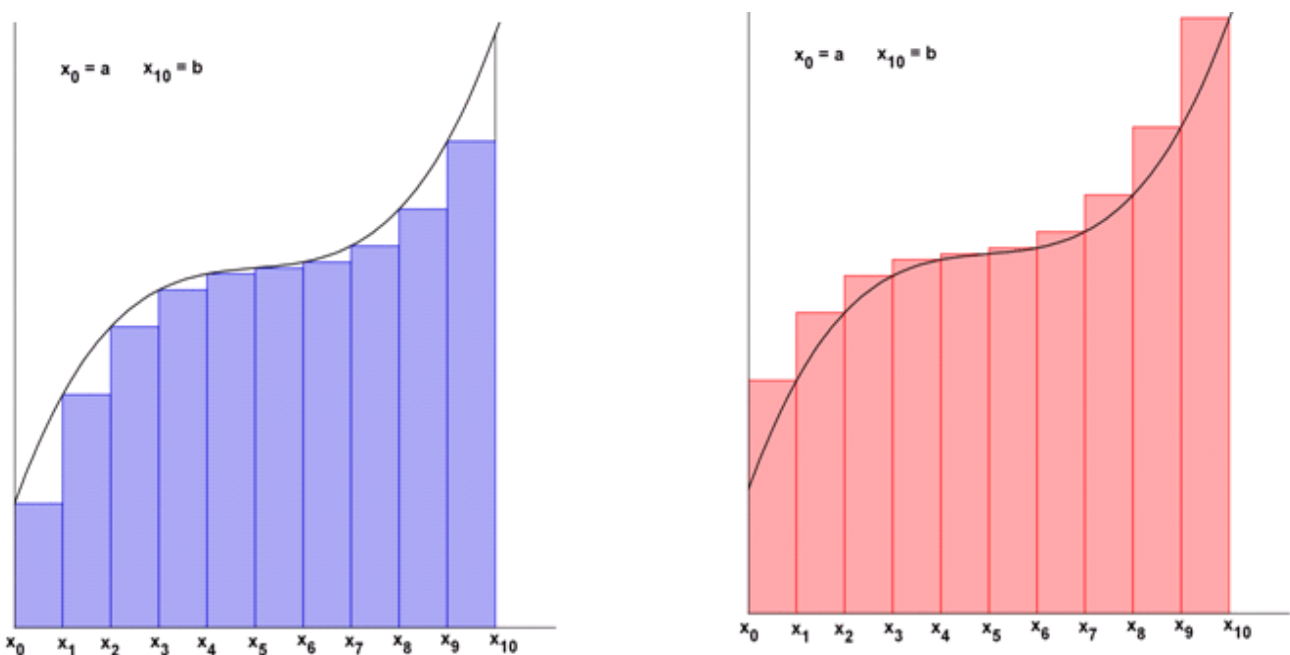
\includegraphics[width=0.8\linewidth]{Bilder/obersumme-untersumme} \\
		
		
		
		\begin{minipage}{0.45\linewidth}
		\textbf{Unter-Integral}		\\
		\\	
		$\underline{I} = \lim \limits_{d(Z) \rightarrow 0} \underline{US} $ \quad \textcolor{blue}{$\infty \cdot 0$} \\
		\\
		$\underline{I} =  \underline{\int \limits_{a}^{b}} f(x) \, dx $ \\
		
		\end{minipage}
		\hfill				
		\begin{minipage}{0.45\linewidth}
		
		
		\textbf{Ober-Integral}		\\
		\\	
		$\overline{I} = \lim \limits_{d(Z) \rightarrow 0} \overline{OS}$ \quad \textcolor{blue}{$\infty \cdot 0$} \\
		\\
		$\overline{I} =  \overline{\int \limits_{a}^{b}} f(x) \, dx $ \\

		\end{minipage}
		
		
		\subsection{Riemann-Summe S.506-507}
		RS = $\sum \limits_{i=0}^{n-1} f(\xi) \Delta x_i$  \quad $d(Z) \rightarrow 0 $ \quad $\int \limits_{a}^{b} f(x) \, dx$ \\
		\\
		$\xi \in [x_i ; x_{i+1}]$		
			
		
		\subsection{Riemann-Integral S.507}
		I = $\underline{I}$ = $\overline{I}$ wenn $\underline{I}$ = $\overline{I}$\\
		\\		
		\begin{minipage}{0.45\linewidth}
		Notation: $ \int \limits_{a}^{b} f(x)\, dx $
		\end{minipage}				
		\hfill
		\begin{minipage}{0.45\linewidth}
		\begin{tabular}{ll}
		$a$, $b$ & Integrationsgrenzen \\
		$f(x)$ & Integrand\\
		\end{tabular}
		\end{minipage}	
		
	
		
		\subsection{Integrierbare Funktionen}
		\textbf{Hinreichendes Kriterium: $f: [a;b] \rightarrow \mathbb{R}$ und $\mathbb{W}_f$ beschränkt}		 \\
		\\	
		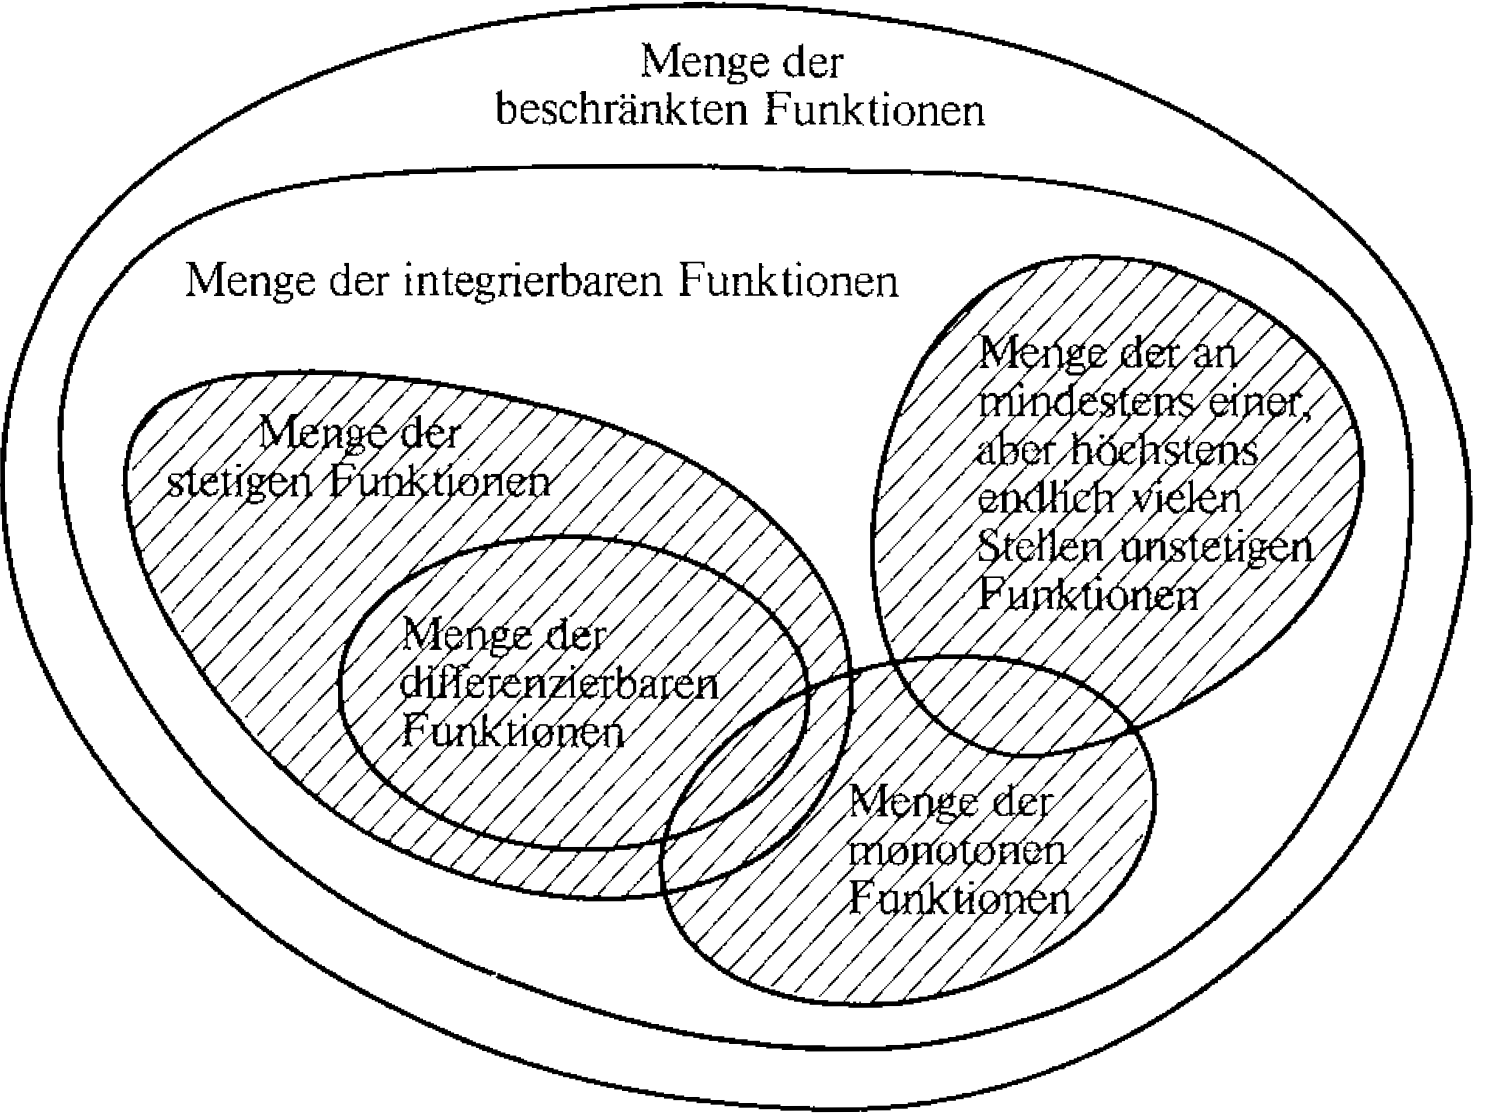
\includegraphics[width=0.7\linewidth]{Bilder/integrierbare-funktionen}
		
		\pagebreak
		
		\subsection{Integrationsregeln S. 494-496}
		Linearität: $\int \limits_{a}^{b} \alpha \, f(x) \, dx = \alpha \int \limits_{a}^{b} f(x)\, dx$ 
		
		
		\subsubsection{Rechenregeln mit Integralen S. 508-510}
		\begin{tabular}{ll}
		Zerlegung: & $\int \limits_{a}^{b} f_1(x) \, dx + f_2(x)\, dx = \int \limits_{a}^{b} f_1(x) \, dx + \int \limits_{a}^{b} f_2(x) \, dx$ \\
		\\		
		& $\int \limits_{a}^{c} f(x)\, dx = \int \limits_{a}^{b} f(x)\, dx + \int \limits_{b}^{c} f(x) \, dx$ \\
		\\
		Grenzen tauschen: & $ \int \limits_{a}^{b} f(x) \, dx = -  \int \limits_{b}^{a} f(x) \, dx $ \\
		\\
		Gleiche Grenzen: &  $\int \limits_{a}^{a} f(x) \, dx = 0$ \\
		\end{tabular}
		
		
		\subsection{Wichtige Integrale S. 495}
		\begin{tabular}{ll}
		$\int \limits_{a}^{b} x^2 \, dx = \frac{b^3}{3} - \frac{a^3}{3}$ & $\int \limits_{a}^{b} x \, dx = \frac{b^2}{2} - \frac{a^2}{2}$ \\
		\\
		$\int \limits_{a}^{b} 1 \, dx = b - a $ (Rechteck)& \\
		\end{tabular}
			
			
		\subsection{Flächen unter Integralen}
		\textbf{Voraussetzung: $f: [a;b] \rightarrow \mathbb{R}$ und $\mathbb{W}_f$ beschränkt}\\
		\\
		Fläche $A = \int \limits_{a}^{b} \vert f(x) \vert \, dx $ \\
		\\
		\textcolor{red}{Der Inhalt des Betrags muss auf Vorzeichen untersucht werden!} \\
		Negative Vorzeichen müssen über die x-Achse geklappt werden: \\
		$\vert x^2 - x \vert = -(x^2 - x)$ falls $x > x^2$ 
		
		
		\subsection{Mittelwert einer Funktion S. 510}		
		Funktion aufgeteilt in n äquidistante Intervalle $\rightarrow \Delta x = \frac{b-a}{n}$ \\
		\\
		Mittelwert: \quad $\frac{1}{b-a} \int \limits_{a}^{b} f(x) \, dx$
		
		
		\subsection{Mittelwertsatz S. 510}
			\textbf{Voraussetzung: $f: [a;b] \rightarrow \mathbb{R}$ und $\mathbb{W}_f$ beschränkt und stetig} \\
		Die Fläche unter der Funktion $f(x)$ kann an mind. einem Punkt $\xi$ als Rechteck dargestellt werden. \\
		$\xi \in (a;b)$ \\
			
		\begin{minipage}{0.40\linewidth}
		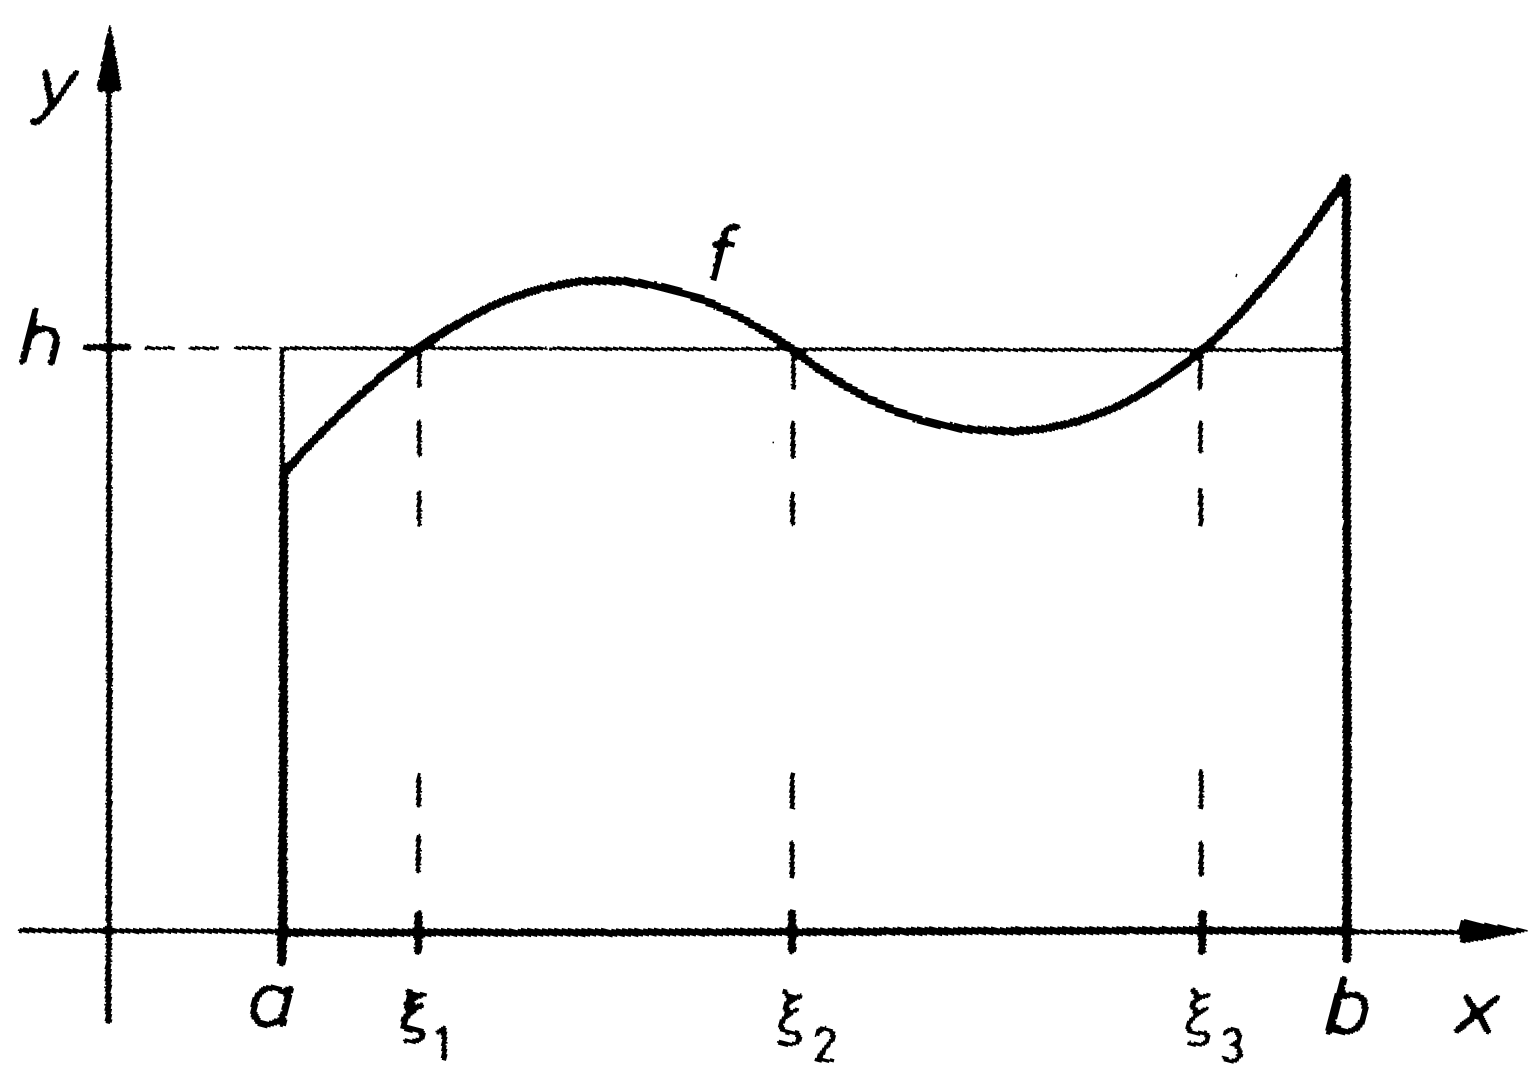
\includegraphics[width=0.95\linewidth]{Bilder/MWS-integral} \\
		\end{minipage}
		\hfill				
		\begin{minipage}{0.55\linewidth}
		
		Fläche =  Mittelwert $\cdot$ Intervall-Länge \\
		\\ 
		 $\frac{1}{b-a} \int \limits_{a}^{b} f(x) \, dx = f(\xi)$ \\
		$ \int \limits_{a}^{b} f(x) \, dx = (b-a) \cdot f(\xi)$ \\
		$ (b-a) \cdot h = (b-a) \cdot f(\xi)$ \\
		\end{minipage}
		
		
		\subsection{Integralfunktion I(x)}
		\textbf{Voraussetzung: $f: [a;b] \rightarrow \mathbb{R}$ und integrierbar} \\
		 \\
		 I(x) besitzt eine feste untere Grenze c = const (Anker) und eine variable obere Grenze x (Hauptvariable) \quad $x \in $[a;b] \qquad  $c \in $[a;b] \\
		 \\
		 Notation: $I(\tilde{x}) = \int \limits_{c}^{x} f(\tilde{x}) d\tilde{x} $  \qquad $\tilde{x}$ ist die Integrationsvariable 
		 
		 
		 \subsubsection{Eigenschaften der Integralfunktion}
			Die Integralfunktion hat beim Anker c eine Nullstelle: \\
			\\
			$I(c) = \int \limits_{c}^{c} f(\tilde{x}) \, d\tilde{x} = 0 $  \\
		\\	
		I(x) berührt/schneidet die x-Achse in [a;b] beim Anker \\
		$\rightarrow$ I(c) = 0 \\
		\\
		Das Verschieben des Ankers bewirkt eine Parallelverschiebung \\ 
		von I(x) \\
		
		\textbf{I(x) ist immer stetig!} (Integration behebt Sprungstellen) \\
		\textbf{I(x) ist ableitbar, \textcolor{red}{wenn die Originalfunktion f(x) stetig ist}}  \\
		\\
		Ableitung $I'(x) = \frac{d}{dx}\left( \int \limits_{c}^{x} f(\tilde{x}) \, d\tilde{x} \right) = f(x)$ \quad "Kreislauf" \\
		\\
		\\
		\begin{tabular}{l c l}
		Integral $I(x)$ &  $\underrightarrow{\text{differenzieren}}$ & $f(x)$ \\
		\\
		Integral $I(x)$ &  $\underleftarrow{\text{integrieren}}$ &  $f(x)$ 
		\end{tabular}
		
		
		\subsubsection{Beispiel Integralfunktion bestimmen}
		$f(x)=\left\{\begin{array}{ll} 1, & 0 \leq x < 0.75 \\
         -0.5, & 0.75 \leq x \leq 2 \end{array} \right.$	\\
     \\
     $I(x)=\left\{\begin{array}{l} \int \limits_{c=0}^{x} 1 \, d \tilde{x} = x \\
     \\
     \textcolor{red}{\int \limits_{c=0}^{0.75} 1 \, d \tilde{x}} + \int \limits_{0.75}^{x} (-0.5) \, d \tilde{x} = 0.75 + (-0.5)(x-0.75)\end{array} \right. $ \\
         	\\
         	\\
         	\textcolor{red}{Wichtig: Bei Funktionen mit Sprungstellen immer beim Anker \\
         	beginnnen, wenn nichts spezielles verlangt ist} \\
         	
         	\columnbreak
         	
		\subsection{Stammfunktion F}
		Eine Funktion $F(x)$ heisst Stammfunktion von $f(x)$ wenn gilt: \\
		\textbf{F'(x) = f(x)} \\
		\\
		$F(x) + C$ sind ebenfalls Stammfunktionen von $f(x)$ \\
		$C \in \mathbb{R}$ \quad C ist eine freie Verschiebungszahl\\
		\\
		Stammfunktionen $F$ sind Teilmenge der unbestimmten Integrale\\
		\\
		$\Rightarrow$ Ableitungstabelle rückwärts lesen für Stammfunktion!
		
		
		\subsection{Unbestimmtes Integral}
			$I(x) + C = \int \limits f(\tilde{x}) \, d\tilde{x} $ \quad  $C \in \mathbb{R}$ \\
			\\
			\textbf{Wenn $f(x)$ stetig ist, dann entspricht das unbestimmte Integral der Stammfunktion}
		
		
		\subsection{Hauptsatz der Integration S. 507}
		$\int \limits_a^b f(x) \, dx = F(b) - F(a) = \left[ F(x) \right]_a^b = F(x) \vert_a^b $
			
	
	
	\subsection{Wachstumsvergleiche}			 
			\begin{tabular}{llll}
			(1) & $\frac{n^k}{q^n} (n \rightarrow \infty)= 0$  & (k $\in \mathbb{N}; q > 1)$ & $\frac{\text{Potenz}}{\text{Exponentiell}} \rightarrow 0$\\
			\\
			(2) & $\frac{q^n}{n!} (n \rightarrow \infty)= 0$ & $(q > 1)$ & $\frac{\text{Exponentiell}}{\text{Fakult"at}} \rightarrow 0$ \\
			\\
			(3) & $\frac{\ln(n)}{n^k} (n \rightarrow \infty)= 0$ & (k $\in \mathbb{N})$ & $\frac{\text{Logarithmisch}}{\text{Potenz}} \rightarrow 0$ \\
			\\
			(4) & $\frac{\ln(n)}{n} (n \rightarrow \infty)= 0$ & & $\frac{\text{Logarithmisch}}{\text{Linear}} \rightarrow 0$ \\
			\end{tabular} %noch nicht kontrolliert

	
	\end{multicols*}	
\end{document}